\documentclass[traditabstract]{aa}
\usepackage{graphicx}
\usepackage[intlimits,sumlimits]{amsmath}
%\usepackage{deluxetable}
\usepackage{times,epsfig} 
\usepackage{natbib}
\usepackage{amssymb}
\bibpunct{(}{)}{;}{a}{}{,} % to follow the A&A style
%for the bibliography at the end
\bibliographystyle{aa} %style aa.bst
\usepackage{amsmath}
\usepackage[english]{babel}

%-------------
\newcommand{\beqa}{\begin{eqnarray}} 

\newcommand{\eeqa}{\end{eqnarray}}
\newcommand{\Abst}[1]{\;#1}
\newcommand{\bsub}{\begin{subequations}}
\newcommand{\esub}{\end{subequations}}
\newcommand{\beal}{\begin{align}}
\newcommand{\ealn}{\end{align}}
\newcommand{\lm}{$L_{max}$~}
\newcommand{\Mni}{$\rm M_{^{56}Ni}$~}
\newcommand{\Ms}{M$_{\sun}$}
\newcommand{\mc}{$\rm M_{Ch}$~}
\newcommand{\Nif}{$
\rm ^{56}Ni$ } 
\newcommand{\Cif}{$\rm ^{56}Co$ }
\newcommand{\Fif}{$\rm ^{56}Fe$}
\newcommand{\ksm}{${\rm km~s^{-1}~Mpc^{-1}}$}
\newcommand{\s}{M$_{\sun}$~}
\begin{document}
%
\title{Reddening-free \Nif estimates for Type Ia supernovae from near infrared data
}


\titlerunning{Nickel mass in SNe~Ia}
\authorrunning{S. Dhawan et al.}
\author{\textbf{Suhail Dhawan\inst{1,2,3}
 	\and B. Leibundgut\inst{1,2}
    \and J. Spyromilio\inst{1}
    \and S. Blondin\inst{4}}}


\institute{European Southern Observatory, Karl-Schwarzschild-Strasse 2, D-85748 Garching bei M\"unchen, Germany \\
\email{sdhawan@eso.org}
\and  Excellence Cluster Universe, Technische Universit\"at M\"unchen,
Boltzmannstrasse 2, D-85748, Garching, Germany\\
\and Physik Department, Technische Universit\"at M\"unchen, James-Franck-Strasse 1, D-85748 Garching bei M\"unchen\\
\and Aix Marseille Universit\'e, CNRS, LAM (Laboratoire d'Astrophysique de Marseille) UMR 7326, 13388 Marseille, France\\
%\email{sdhawan@eso.org}
} 

\date{Received; accepted }

\offprints{S. Dhawan}

\abstract{The population of Type Ia supernovae (SNe\,Ia) exhibits a significant diversity. The reasons (e.g. parent population, explosion mechanism) for this diversity remain largely unknown.
Using a sample of 18 SNe\,Ia with  low absorption by the host galaxy, we investigate the relation between the UVOIR peak luminosity  $L_{max}$ and the phase of the second maximum ($t_2$) and find a very tight correlation. 

The $L_{max}$ vs. $t_2$ relation is applied to a sample of 40 additional SNe\,Ia with significant reddening ($E(B-V) >$ 0.1 mag) and a reddening-free bolometric luminosity function of SNe\,Ia is established. The $L_{max}$ is used to derive the \Nif masses for both the unreddened and reddened samples. The method is tested with the \Nif mass measurement from the direct observation of $\gamma-$rays in the heavily absorbed SN~2014J and found to be fully consistent. 

Super-Chandrasekhar-mass explosions, in particular SN\,2007if, do not follow the relations between peak luminosity and second IR maximum. This may point to additional energy created during the maximum light period and hence violating Arnett's rule.
{\bf JSP: I am not sure I understand this statement}

The luminosity function of SNe\,Ia is constructed and is shown to be asymmetric with a tail of low-luminosity objects and a rather sharp high-luminosity cutoff although this may be due to selection effects. Using this method, the nickel mass function of SNe\,Ia shows a large dispersion of over a factor 2. This is a lower limit as our sample did not include low-luminosity SNe\,Ia, which do not show a second maximum.}%{junk}{junk}{junk}{junk}

%\abstract{}{To determine the relation between the total amount of radioactive Nickel ($^{56}Ni$) produced in Type Ia supernovae (SNIa) and the timing of the second maximum ($t_2$) in the Near Infrared (NIR; $YJH$) bands and to  extrapolate Nickel mass values for reddened SNIa using this relation} 
%{We measure the  (pseudo)-bolometric luminosity at peak from the ultraviolet optical Near Infrared (UVOIR) light curves  and use it to derive a value for the amount of $^{56}Ni$ produced ($M_{^{56}Ni}$) for a  sample of objects with very little reddening from the host galaxy.Therefore, the effects from presuming a reddening law are smaller.  }
%{We find a strong correlation between the peak bolometric luminosity ($L_{max}$) and $t_2$ in the $Y$ and $J$ bands and a weaker trend in the $H$ band. We use this empirical relation to derive $L_{max}$ and therefore,  $M_{^{56}Ni}$ for test case SNae with high extinction. This allows us to have a $M_{^{56}Ni}$ value which is independent of the reddening law applied. We also apply the relation to all objects not in the low-reddening sample for which a $t_2$ is measured.}
%{From our results we conclude that an empirical relation between  $L_{max}$ and $t_2$ can allow us to infer the  $M_{^{56}Ni}$.The estimates from this method for nearby highly reddened SNae are consistent with independent estimates in the literature. Using the $t_2$ parameter, we measure the $L_{max}$ for a large sample of SNe and conclude that they have a diverse range of bolometric peaks, and hence a range of $M_{^{56}Ni}$ indicating a significant variation in the explosion mechanism}




%%-----------------
\keywords{supernovae:general -- supernovae: individual:2014J, 2006X} %
\maketitle
\section{Introduction}
\label{sec-intro}

Type Ia supernovae (SNe\,Ia) exhibit diverse observable properties. In addition to the spectral and colour differences, the peak luminosity of SNe\,Ia  range over several factors \citep[e.g.][]{Suntzeff1996, Suntzeff2003, Li2011}. The amount of $^{56}$Ni, derived from the bolometric luminosity, \citep{Contardo2000} and the total ejecta mass \citep{Stritzinger2006a, Scalzo2014} also show a wide dispersion. The $M_{^{56}Ni}$ distribution provides insight into the possible progenitor channels and explosion mechanisms for SNe\,Ia \citep[see][]{Hillebrandt2000, Livio2000, Truran2012}.

%\Mni can, in principle, be derived from the peak luminosity of multi-band ("pseudo-bolometric") light curves . 
Following \citet{Arnett1982} at the epoch of maximum light the luminosity corresponds approximately to the the instantaneous energy input from the \Nif decay chain and therefore is a powerful tool for the determination of the mass of \Nif.  The method is limited, in part, by the accuracy of the correction for reddening in the Milky Way and the host galaxy. The total to selective absorption ($R_V$) appears systematically and significantly lower in the SN hosts than the canonical Milky Way $R_V$ value of 3.1. \citet{Nobili2008} used a large sample of nearby SNe\,Ia to derive an average $R_V$ which is significantly lower than 3.1. Taking into account spectroscopic features that correlate with luminosity \citet{Chotard2011} found a more 'normal' $R_V$ of $2.8 \pm 0.3$. However,  objects with high extinction are seen to have an unusually low $R_V$ \citep{Phillips2013, Patat2014}. To remove this uncertainty, we aim to establish a relation between the \Nif mass and observed properties of SN\,Ia in order to establish a \Nif mass distribution independent of reddening. %We present here a relation between the phase of the second maximum in the infrared light curves of SNe~Ia and the nickel mass, which is independent of reddening and allows us to establish the nickel mass distribution among SN~Ia explosions.

%Near infrared (NIR) observations of SNe\,Ia provide a promising new approach, which was mostly advocated for improved distance measurements \citep{Meikle2000, Krisciunas2007, Wood-Vasey2008, Barone-Nugent2012}. The uniformity of the NIR peak luminosities together with the reduced effect of absorption yield distances with the uncertainties of light curve fitting and reddening corrections essentially removed. 
%NIR light curves provide interesting clues on the physics of the explosions.  In particular the rebrightening of SNe\,Ia about 2 weeks after the first maximum holds interesting information on the \Nif produced in the explosions \citep{Dhawan2015}. 
The Near Infrared (NIR) light curve morphology of SNe\,Ia differs from that in the optical. In particular, the light curves start to rebrighten about 2 weeks after the optical maximum, resulting in a second peak. 
Recent studies \citep[e.g.][]{Biscardi2012,Dhawan2015}  found that more luminous SNe\,Ia reach the second maximum in NIR  filters at a later phase as predicted by \citet{Kasen2006} who also indicated that the phase of the second maximum should be a function of the \Nif mass in the explosion.  We, therefore, would expect that the phase of the second NIR maximum can be used to determine the amount of \Nif  synthesized in the explosion. 

In the following, we investigate the link between the peak bolometric luminosity ($L_{max}$) and the phase of the second maximum in the NIR light curves ($t_2$). We use a sample of nearby low-absorption objects (described in Section~\ref{sec-data}) to determine the relation using different methods to derive $M_{^{56}Ni}$ (Section~\ref{sec-res}). We then apply this relation to derive $M_{^{56}Ni}$ for all SNe\,Ia in our sample with a measured $t_2$. In Section~\ref{sec-test} we check our derivation using two supernovae with independent measurements of $M_{^{56}Ni}$ (SN\,2014J  and SN\,2006X) . Using this reddening independent method we can establish the luminosity function of SNe\,Ia at maximum and also derive the distribution of nickel masses among SN\,Ia explosions (Section~\ref{sec-lfunc}). We discuss the implications of this determination of the $M_{^{56}Ni}$ distribution in the conclusions (Section~\ref{sec-dnc}).

\begin{figure}
\centering
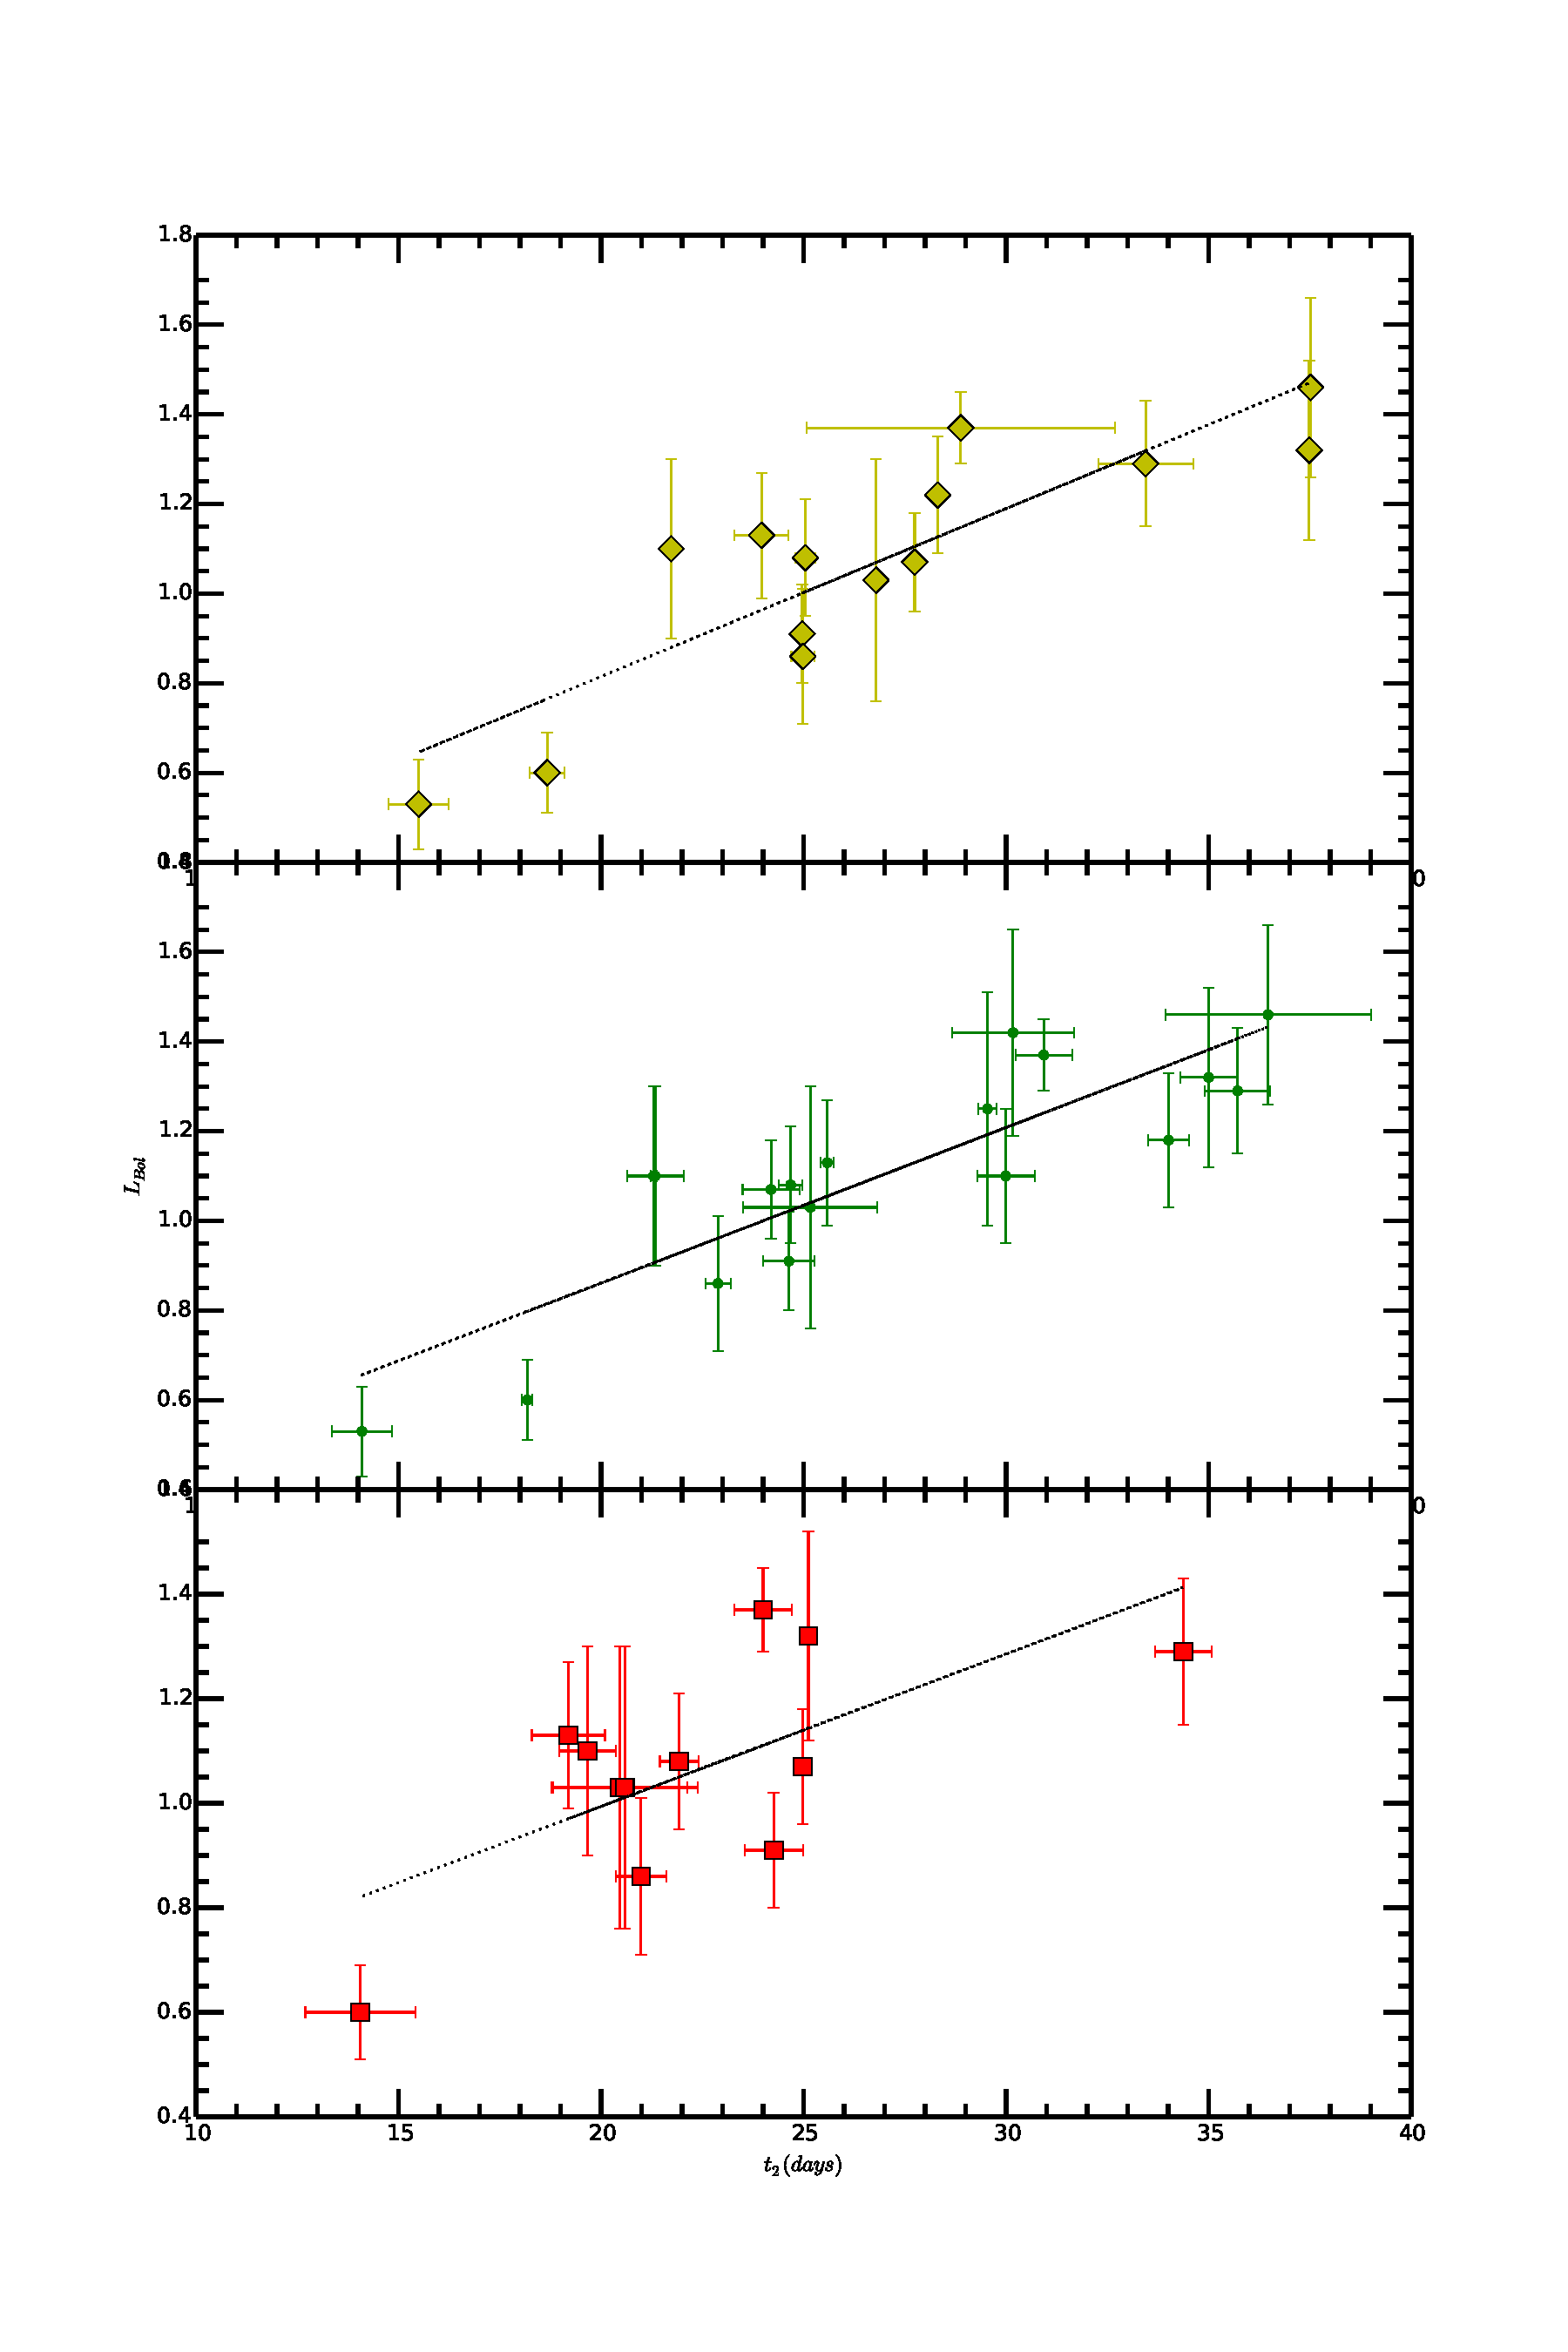
\includegraphics[width=.50\textwidth, height=0.6\textheight]{lbolt2_bf.pdf}
\caption{The bolometric maximum luminosity $L_{max}$ is plotted against the phase of the second maximum $t_2$ in $YJH$ filter light curves. A strong correlation is observed in  $Y$ and $J$, whereas a weaker correlation is seen in the $H$ band.  Best fit lines are overplotted in black. The fit includes errors on both axes. Black points are the values from the DDC models \citep{Blondin2013}.}
\label{fig:nit2}
\end{figure}


\section{Data} 
\label{sec-data}

From the photometry pblished by the Carnegie Supernova Project \citep[CSP;][]{ Contreras2010,Burns2011,Stritzinger2011,Phillips2012,Burns2014} we select SN\,Ia which have NIR observations at late times ($t>50$ days after B maximum) and with well-sampled optical and NIR light curves allowing us to determine an accurate $t_2$ and construct (pseudo-)bolometric light curves. We add to this sample objects from the literature that meet the same criteria. The full description of the selected SNe\,Ia can be found in \citet{Dhawan2015}.

A sample of 18 low-reddening ( $E(B-V)_{host}<0.1$ mag) SNe\,Ia is presented in Table~\ref{tab:lr}. We use $E(B-V)_{host}$ values from the literature. These values are calculated from SN light curve fits. {\bf JSP: these two sentences together make no sense.} Since we only included supernovae, which display the second maximum in their NIR light curves this implies that most low-luminosity SNe\,Ia, especially SN\,1991bg-like objects were also excluded.

The integrated flux emitted by an SN\,Ia in the UV, optical and NIR traces the comptonization of the $\gamma-$rays emitted through the \Nif $\rightarrow$  $^{56}$Co $\rightarrow$ $^{56}$Fe decay chain \citep[e.g.][]{Nadyozhin1994} {\bf JSP: this is a funny set of references for this science plus I think that what you are trying to say is what is in the next sentence and therefore I would skip the previous one}.
At maximum light the UV-optical-IR integrated luminosity represents 94 $\%$ of the true bolometric luminosity \citep{Blondin2015}. 
%As the SN emits most of its flux in the UV to NIR passbands, the "UVOIR bolometric flux" represents a physically meaningful quantity \citep{Suntzeff1996, Contardo2000}.

We constructed $UBVRIJH$ bolometric light curves for objects with sufficient photometry near maximum light in the optical and the NIR. The $K$ band data was not included since only few SN\,Ia have well-sampled $K$ light curves. We calculated the fraction of the flux emitted in $K$ for a few well-observed SNe\,Ia with sufficient data and determined it to be around $1-3 \%$ of the UVOIR luminosity at maximum. Therefore, the exclusion of the $K$-flux results in only a minor uncertainty in the final UVOIR luminosity.  
%{\bf during which phase? maximum?}
The small reddening correction {\bf JSP: this is all very confused in the text. } following \citet{Cardelli1989} was applied to our data before integrating over the available passbands and the uncertainty propagated into the bolometric flux. We use a distance scale of $H_0=70$~$km$~$s^{-1}$~$Mpc^{-1}$ {\bf JSP: this is the same comment as in the other paper. Just reference the distance papers or NED} and the assumed distances are indicated in Table~\ref{tab:mni}. For the nearby SN\,Ia with distance measurements provided through direct methods (e.g. Cepheid stars, Tully-Fisher relation) we made sure to employ the same distance scale. 

{\bf JSP proposed replacement text  from {\em The small ...} to {\em distance scale}} {\it Prior to the  derivation of a bolometric flux for the low extinction sample (see Table~\ref{tab:mni}) we apply a correction for the measured extinction following \citet{Cardelli1989}. The distances assumed for the sample and references can be found in Table~\ref{tab:mni}}  

SN2008gp	&	35.79	&	0.06		&	$0.098(0.022)$	&	0.104(0.005)	& UBVRIJH	\\
%SN2008bq	&	0.78	&	0.23	&	1.18	&	$0.136(0.027)$	&	0.077(0.002)	&	\\
SN2007as	&	34.45	&	0.12		&	$0.050(0.011)$	&	0.123(0.001)	& UBVRI	\\
SN2008bc	&	34.16	&	0.13		&	$<0.019$	&	0.225(0.004)	& UBVRIJH	\\
%SN2004gs	&	0.37	&	0.05	&	0.54	&	$0.148(0.024)$	&	0.026(0.001)	&	\\
SN2008hv	&	33.84	&	0.15			&	$0.074(0.023)$	&	0.028(0.001)	& UBVRIJH	\\
SN2008ia	&	34.96	&	0.09		&	$0.066(0.016)$	&	0.195(0.005)	& UBVRIJH	\\
SN2005na	&	35.34	&	0.08		&	$0.061(0.022)$	&	0.068(0.003)	& UBVRI	\\
SN2005eq	&	35.46	&	0.07		&	$0.044(0.024)$	&	0.063(0.003)	& UBVRIJH	\\
%SN2006D		&	0.57	&	0.08	&	0.93	&	$0.134(0.025)$	&	0.039(0.001)	&	\\
SN2005M		&	35.01	&	0.09		&	$0.060(0.021)$	&	0.027(0.002)	& UBVRIJH	\\
SN2007on	&	31.45	&	0.08		&	$<0.007$	&	0.010(0.001)	& UBVRIJH	\\
SN2007nq	&	36.44	&	0.05		&	$0.046(0.013)$	&	0.031(0.001)	& BVRI	\\
SN2005am	&	32.85	&	0.20		&	$0.053(0.017)$	&	0.043(0.002)	& UBVRIJH	\\
SN2005hc	&	36.50	&	0.05		&	$0.049(0.019)$	&	0.028(0.001)	& UBVRIJH	\\
%SN2005ke	&	0.13	&	0.1	&	0.26	&	$0.263(0.033)$	&	0.020(0.002)	&	\\
SN2004gu	&	36.59	&	0.04		&	$0.096(0.034)$	&	0.022(0.001)	& BVRI	\\
SN2011fe	&	28.91	&	0.20		&	$0.03 (0.01)$	&	0.021(0.001)	& UBVRIJH	\\
SN2001ba	&	35.40	&	0.50		&	$ 0.010 (0.04)$  &     0.021 (0.002)	& UBVRIJH	\\
SN2002dj	&	31.70	&	0.30		&	$   0.020 (0.03)$ & 0.080 (0.003)		& UBVRIJH		\\
SN2002fk	&	32.59	&	0.15		&	$0.030 (0.01)$   & 0.030 (0.003)		& UBVRIJH 				\\
SN2008R		&	33.73	&	0.16		&  $0.009(0.013)$ & 0.062(0.001)          & 	UBVRIJH		\\
SN2005iq	&	35.80	&	0.15		& $0.040(0.015)$ & 0.019(0.001) & UBVRIJH	\\	
SN2005ki	&	34.73	&	0.10		& $0.016(0.013)$ & 0.027(0.001) & UBVRIJH	\\
SN2006bh	&	33.28	&	0.20		& $0.037(0.013)$ & 0.023(0.001) & UBVRIJH	\\
SN2007bd	&	35.73	&	0.07		&  $0.058(0.022)$ & 0.029(0.001)        & UBVRIJH	\\




%-------------------------------------------------------
%%%INPUTS FOR ANALYSIS, RESULTS, DISCUSSION
%-----------------------------------------------------

%\section{Analysis}
%\label{sec-ana}
%The flux emitted by an SNIa in the UV, optical and NIR traces the comptonization of the photons emitted through the $^{56}$Ni $\rightarrow$  $^{56}$Co $\rightarrow$ $^{56}$Fe decay chain \citep[see][]{Nadyozhin1994}.
As the SN emits most of its flux in the UV to NIR passbands, the "uvoir bolometric flux" represents a physically meaningful quantity \citep{Suntzeff1996}

We select a low-reddening sample with objects that have a host extinction less than $0.1 mag$. This makes our measurements are less sensitive to a reddening law. 
For objects with sufficient amount of near maximum data in the optical and the NIR, we construct UBVRIJH bolometric light curves. We do not use $K$ band data since there are very few objects in the sample with well-sampled $K$ band light curves. Using  objects that have well-sampled $K$ light curves we calculate the flux emitted in the $K$ band and find that it is between $1-3 \%$. Thus, not using the $K$-band is not a dominant source of uncertainty. 
The magnitudes were corrected 
for reddening using a CCM reddening law for each filter. The values for the extinction are presented in table \ref{tab:mni}. The uncertainty in the reddening estimate
was propagated into the calculation of the bolometric flux
Using zero-points in the given filters, the magnitudes were converted to fluxes. The data in the different filters is interpolated, instead of using a reference filter. The filters are integrated using the trapezoidal rule.
The resulting light curve, in ergs/$cm^2$/s  was converted into an absolute bolometric light curve 
by using the distances of the SN derived from the host galaxy redshift. 

Since all distances are scaled to an $H_0=70 km s^{-1} Mpc ^{-1}$the errors in the luminosity distance are only affected by the relative errors in the 
distance moduli (see Table \ref{tab:mni} for values and uncertainty estimates). For objects not in the hubble flow, we use distance measurements from published estimates (which use others methods eg. Cepheid, Tully-Fisher relation etc.). 

In our sample, for uniformity, we restrict the analysis to objects with coverage from $u-H$ bands with coverage around the bolometric peak.

SN2008gp	&	35.79	&	0.06		&	$0.098(0.022)$	&	0.104(0.005)	& UBVRIJH	\\
%SN2008bq	&	0.78	&	0.23	&	1.18	&	$0.136(0.027)$	&	0.077(0.002)	&	\\
SN2007as	&	34.45	&	0.12		&	$0.050(0.011)$	&	0.123(0.001)	& UBVRI	\\
SN2008bc	&	34.16	&	0.13		&	$<0.019$	&	0.225(0.004)	& UBVRIJH	\\
%SN2004gs	&	0.37	&	0.05	&	0.54	&	$0.148(0.024)$	&	0.026(0.001)	&	\\
SN2008hv	&	33.84	&	0.15			&	$0.074(0.023)$	&	0.028(0.001)	& UBVRIJH	\\
SN2008ia	&	34.96	&	0.09		&	$0.066(0.016)$	&	0.195(0.005)	& UBVRIJH	\\
SN2005na	&	35.34	&	0.08		&	$0.061(0.022)$	&	0.068(0.003)	& UBVRI	\\
SN2005eq	&	35.46	&	0.07		&	$0.044(0.024)$	&	0.063(0.003)	& UBVRIJH	\\
%SN2006D		&	0.57	&	0.08	&	0.93	&	$0.134(0.025)$	&	0.039(0.001)	&	\\
SN2005M		&	35.01	&	0.09		&	$0.060(0.021)$	&	0.027(0.002)	& UBVRIJH	\\
SN2007on	&	31.45	&	0.08		&	$<0.007$	&	0.010(0.001)	& UBVRIJH	\\
SN2007nq	&	36.44	&	0.05		&	$0.046(0.013)$	&	0.031(0.001)	& BVRI	\\
SN2005am	&	32.85	&	0.20		&	$0.053(0.017)$	&	0.043(0.002)	& UBVRIJH	\\
SN2005hc	&	36.50	&	0.05		&	$0.049(0.019)$	&	0.028(0.001)	& UBVRIJH	\\
%SN2005ke	&	0.13	&	0.1	&	0.26	&	$0.263(0.033)$	&	0.020(0.002)	&	\\
SN2004gu	&	36.59	&	0.04		&	$0.096(0.034)$	&	0.022(0.001)	& BVRI	\\
SN2011fe	&	28.91	&	0.20		&	$0.03 (0.01)$	&	0.021(0.001)	& UBVRIJH	\\
SN2001ba	&	35.40	&	0.50		&	$ 0.010 (0.04)$  &     0.021 (0.002)	& UBVRIJH	\\
SN2002dj	&	31.70	&	0.30		&	$   0.020 (0.03)$ & 0.080 (0.003)		& UBVRIJH		\\
SN2002fk	&	32.59	&	0.15		&	$0.030 (0.01)$   & 0.030 (0.003)		& UBVRIJH 				\\
SN2008R		&	33.73	&	0.16		&  $0.009(0.013)$ & 0.062(0.001)          & 	UBVRIJH		\\
SN2005iq	&	35.80	&	0.15		& $0.040(0.015)$ & 0.019(0.001) & UBVRIJH	\\	
SN2005ki	&	34.73	&	0.10		& $0.016(0.013)$ & 0.027(0.001) & UBVRIJH	\\
SN2006bh	&	33.28	&	0.20		& $0.037(0.013)$ & 0.023(0.001) & UBVRIJH	\\
SN2007bd	&	35.73	&	0.07		&  $0.058(0.022)$ & 0.029(0.001)        & UBVRIJH	\\









\section{Results}
\label{sec-res}
In this section we present the results derived from the measurements of the peak bolometric luminosity and the trends observed with other parameters for the SNe in our low-reddening sample. We also extend the analysis to the complete sample of objects with a measured second maximum.


\begin{table*}
\caption{$L_{max}$ measurements for low reddening SNIa with a measured $t_2$. }

\begin{center}
\begin{tabular}{llccccrrr}
\hline
SN  & $L_{max}(\cdot e^{43} erg s^{-1})$ & $e_{L}$  & $M_{Ni}-Arn (M_{\odot})$  & $M_{Ni}-Arn (M_{\odot})$ (fixed rise)  & $M_{Ni}-DDC (M_{\odot})$\\% & $E(B-V)_{MW}$ & u-band lum \\
\hline
%SN2001ba & 1.18 & 0.15 & 0.58 & 0.59 & 	0.57 \\
SN2002dj & 1.25 & 0.26 & 0.59 & 0.63 & 0.61 \\
SN2002fk & 1.42 & 0.23 & 0.68 & 0.71 & 0.76 \\
SN2005M & 1.37 & 0.08 & 0.70 & 0.69 & 0.71 \\
SN2005am & 1.1 & 0.2 & 0.47 & 0.55 & 0.52 \\
SN2005el & 0.91	& 0.11 & 0.40 & 0.46   & 0.44 	\\	
SN2005eq & 1.32 & 0.2 & 0.67 & 0.66 & 0.67 \\
SN2005hc & 1.36 & 0.2 & 0.69 & 0.68 & 0.71 \\
SN2005iq & 1.07 & 0.11 & 0.48 & 0.54 & 0.51 \\
SN2005ki & 1.03 & 0.27 & 0.45 & 0.51 & 0.49 \\
SN2006bh & 0.86 & 0.15 & 0.37 & 0.43 & 0.40 \\
SN2007bd & 1.22 & 0.13 & 0.55	  & 0.61 & 0.59	\\
SN2007on & 0.6 & 0.09 & 0.24 & 0.30 & 0.28 \\
SN2008R & 0.53 & 0.1 & 0.21 & 0.26 & 0.25 \\
SN2008bc & 1.24 & 0.19 & 0.60 & 0.62 & 0.63 \\
SN2008gp & 1.29 & 0.14 & 0.62 & 0.65 & 0.64 \\
SN2008hv & 1.08 & 0.13 & 0.48 & 0.54 & 0.52 \\
SN2008ia & 1.13 & 0.14 & 0.50 & 0.57 & 0.55 \\
SN2011fe & 1.1 & 0.15 & 0.50 & 0.55 & 0.52 \\
\hline
\end{tabular}
\label{tab:mni}
\end{center}
\end{table*}

\subsection{Correlation between $L_{max}$ and $t_2$ }

In figure ~\ref{fig:nit2}, we find that there is a very strong correlation between $t_2$ and $M_{^{56}Ni}$ in the $Y$ and $J$ bands with $r$ values of 
0.80, 0.88. A much weaker trend is observed in the $H$ band with $r \sim$ 0.60. This is reflected in the ratio of the slope to the slope error in equation \eqref{eq:lin_t2}

\begin{table}
\caption{Values of the coefficients for correlations between $L_{max}$ and $t_2$ in the individual filters}
\begin{center}
\begin{tabular}{llcc}
\hline
Filter & $a_i $ & $b_i $	 \\
\hline
Y    &	0.043($\pm$0.005)  &	-0.100($\pm$0.133)	\\
J    & 	0.040($\pm$0.004)  &	-0.047($\pm$0.118)		\\
H    & 	0.036($\pm$0.009)  &	 0.256($\pm$0.222)		\\
\hline
\end{tabular}
\end{center}
\label{tab:coeff}
\end{table}


In the $Y$ and $J$ band, a strong correlation suggests that objects with more Ni produced show later second maxima. 
\begin{equation}
\label{eq:lmt2}
L_{max}=a_i \cdot t_2(i) + b_i
\end{equation}

From Table ~\ref{tab:coeff} and figure \ref{fig:nit2}, we can see that the constraints on the slope for the best fit relation in the $H$ band are weak. Hence, for further analyses, we do not use the $H$ band.

Equation \eqref{eq:lmt2} relates $t_2$ to the bolometric luminosity. The coefficients for the linear fit and the errors on the estimates are given in Table ~\ref{tab:coeff}. 
%Equations \eqref{eq:ly,eq:lj,eq:lh} relate the timing of the second maximum to the peak bolometric luminosity by combining equation \eqref{eq:eni} with equation \eqref{eq:y,eq:j,eq:h}. We can see that the relation is dependent on the rise time of the SN and the $\alpha$ parameter which encodes the deviation from Arnett's rule.

%From the equations it is evident that the timing of the second maximum in $H$ doesn't provide stringent constraints on the bolometric peak luminosity.
\subsection{Low galactic reddening sample}
In our sample, we selected objects with a host galaxy extinction $<$ 0.1 mag. For some of these objects, the galactic extinction is $>$ 0.1 mag. In order to see whether these objects influence the strength of the correlation, we evaluate the correlation coefficients for a sample without the high galactic reddening objects.
 As a result, 7 objects with $E(B-V)_{host}<$0.1 but total E(B-V) $\geq$ 0.1 are removed. We do not find a substantial decrease in the correlation coefficients in the $YJH$ bands, which are 0.76, 0.83, 0.60 respectively. Since we know the reddening law in the MW with high certainty, we can correct the bolometric light curves for the absorption from the MW dust. Thus, for further analysis we do not truncate the sample from the original low reddening objects in Table ~\ref{tab:lr}




\subsection{Deriving $M_{^{56}Ni}$ from $L_{max}$}
\label{ssec-derni}
In the sections above, we have found a strong correlation between $L_{max}$ and $t_2$ in the $Y$ and $J$ bands. 
%From this correlation we have derived a value for the peak bolometric luminosity of a sample of 5 highly reddened supernovae, which we have summarised in Table ~\ref{tab:red}.

Since our final aim is to derive a value of the $^{56}Ni$ mass for objects which have a measured value of $t_2$, we present the different methods to derive $M_{^{56}Ni}$ from the peak bolometric luminosity.

In figure \ref{fig:nicomp}, we plot the distributions of the $M_{^{56}Ni}$ from the different methods.
\subsubsection{Arnett's rule with a variable rise time}
Arnett's rule states that the luminosity of the SN at peak is given by the instantaneous rate of energy deposition from radioactive decays inside the expanding ejecta. 
This is summarized in equation \eqref{eq:lm-eni}. 
\begin{equation}
L_{max}=\alpha E_{Ni} (t_R)
\end{equation}

Where $E_{Ni}$ is the input from $^{56}$Ni decay at maximum, $t_R$ is the rise time and $\alpha$ accounts for deviations from Arnett's Rule.

\begin{equation}
\label{eq:eni}
E_{Ni} (1 M_{\odot})= 6.45  \cdot 10^{43} e^{-t_R/8.8} + 1.45  \cdot  10^{43} e^{-t_R/111.3}
\end{equation}

For estimates using different rise times, we follow the relation in \citet{G2011}
\begin{equation}
t_{R, B}=17.5 - 5(\Delta m_{15} - 1.1)
\end{equation}
and  
\begin{equation}
t_{R, Bol}=t_{R, B}+ (t_{max, bol} -t_{max, B})
\end{equation}
which implies 

\begin{multline}
L_{max}=\alpha \cdot (6.45  \cdot  10^{43} e^{-(t_{R, bol}/8.8}) + \\ 1.45  \cdot  10^{43} e^{-t_{R,bol}/111.3})  \cdot(M_{Ni}/M_{\odot})
\end{multline}

substituting the relation derived between $L_{max}$ and $t_2$ (equation \eqref{eq:lmt2}) we get a relation between $t_2$ and $M_{^{56}Ni}$

\begin{equation}
\label{eq:nit2}
M_{^{56}Ni}= \frac{a_i \cdot t_2(i) + b_i}{\alpha \cdot E_{Ni}(t_2(i))} 
\end{equation}

From equation \eqref{eq:nit2}, we can see that the relation between $M_{^{56}Ni}$ and $t_2$ is non-linear.  

 
\subsubsection{Arnett's rule with a fixed rise time}
For this method of deriving $M_{^{56}Ni}$ from $L_{max}$, we use a fixed rise time of 19 days, as in \citet{Stritzinger2006}. Similar to their analysis, we propagate an uncertainty of $\pm$ 3 days 
\begin{equation}
\label{eq:arn}
L_{max}=(2.0 \pm 0.3) \cdot 10^{43} (M_{^{56}Ni}/M_{\odot}) erg s^{-1}
\end{equation}

For deriving equation \eqref{eq:arn} we need to use a specific value of $\alpha$. In previous studies \citep[eg.][]{Stritzinger2006,Mazzali2007}, the authors use $\alpha$=1. This value is very close to the self consisent models of \citet{Arnett1982} and is also the mean values for the models of \citet{Hoeflich1995}. Hence, in our study, we use $\alpha$=1.

From the DDC models, we calculate the ratio of decay energy to the bolometric luminosity (which is the $\alpha$ value) for the different $M_{^{56}Ni}$ input values. We find that the values have a mean of 1.03 with a $\sigma$ of 0.07. We find that these values are consistent with the simplifying assumption that $\alpha$=1.
  
\begin{figure}
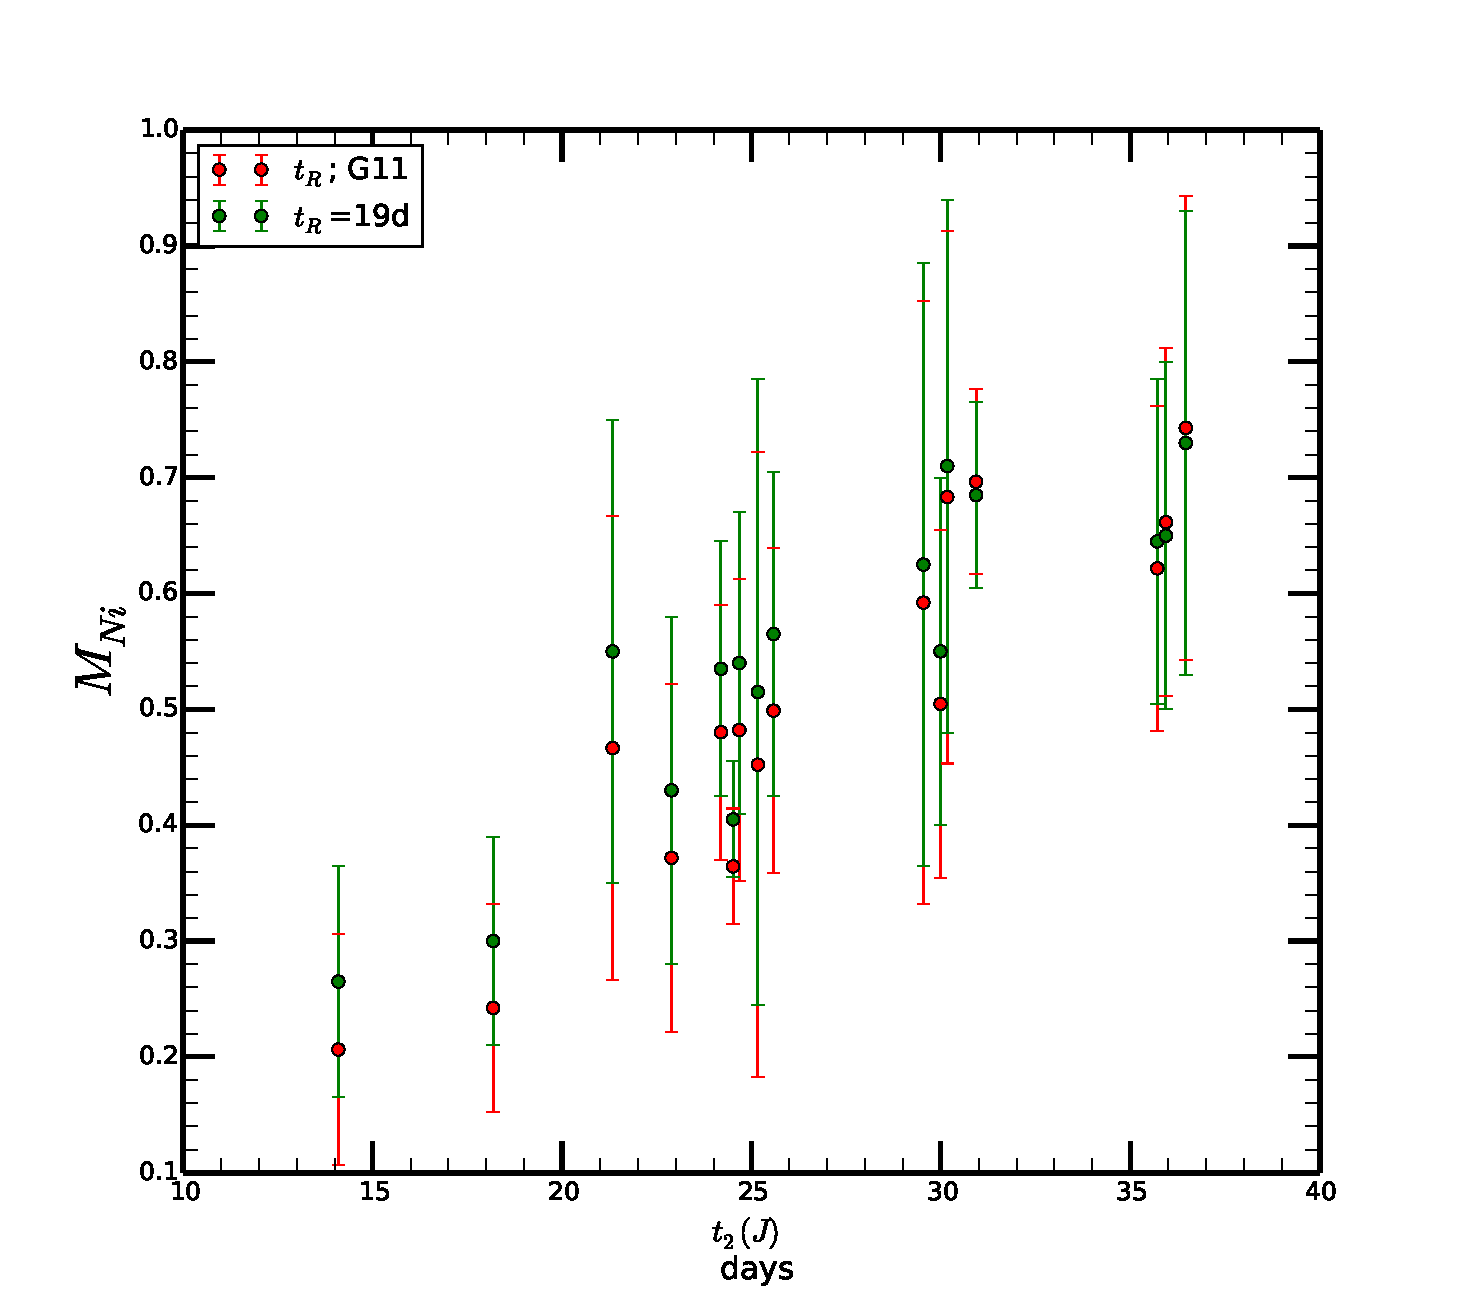
\includegraphics[width=.5\textwidth, trim= 0 30 0 30]{../plot_rel/comp_tr_nit2.pdf}
\caption{Comparison of the $M_{^{56}Ni}$ versus $t_2$ relations for using Arnett's rule with variable (\emph{red circles}) and fixed (\emph{green circles}) rise time. }
\end{figure}

%----------------------------------%

\subsubsection{Interpolating using DDC models}
Another possible method for deriving   $M_{^{56}Ni}$ values from $L_{max}$ is by interpolating the relation found from theoretical models between these two quantities. In our analysis, we use the DDC models from \citet{Blondin2013} as another method of obtaining $M_{^{56}Ni}$.

For objects without NIR coverage, these models can be used to calculate the $M_{^{56}Ni}$-$L_{max}$ relationship for a set of optical-only filters (eg. SN2004gu only has $BVRI$ coverage near maximum). 
This method, therefore, has the advantage of being able to derive $M_{^{56}Ni}$ values for objects with missing passbands without an additional correction term applied to the $L_{max}$. However, in order to keep the samples uniform across the different methods, we only use the objects with complete coverage from $u$ ot $H$ bands. 

%----------%

\begin{figure}
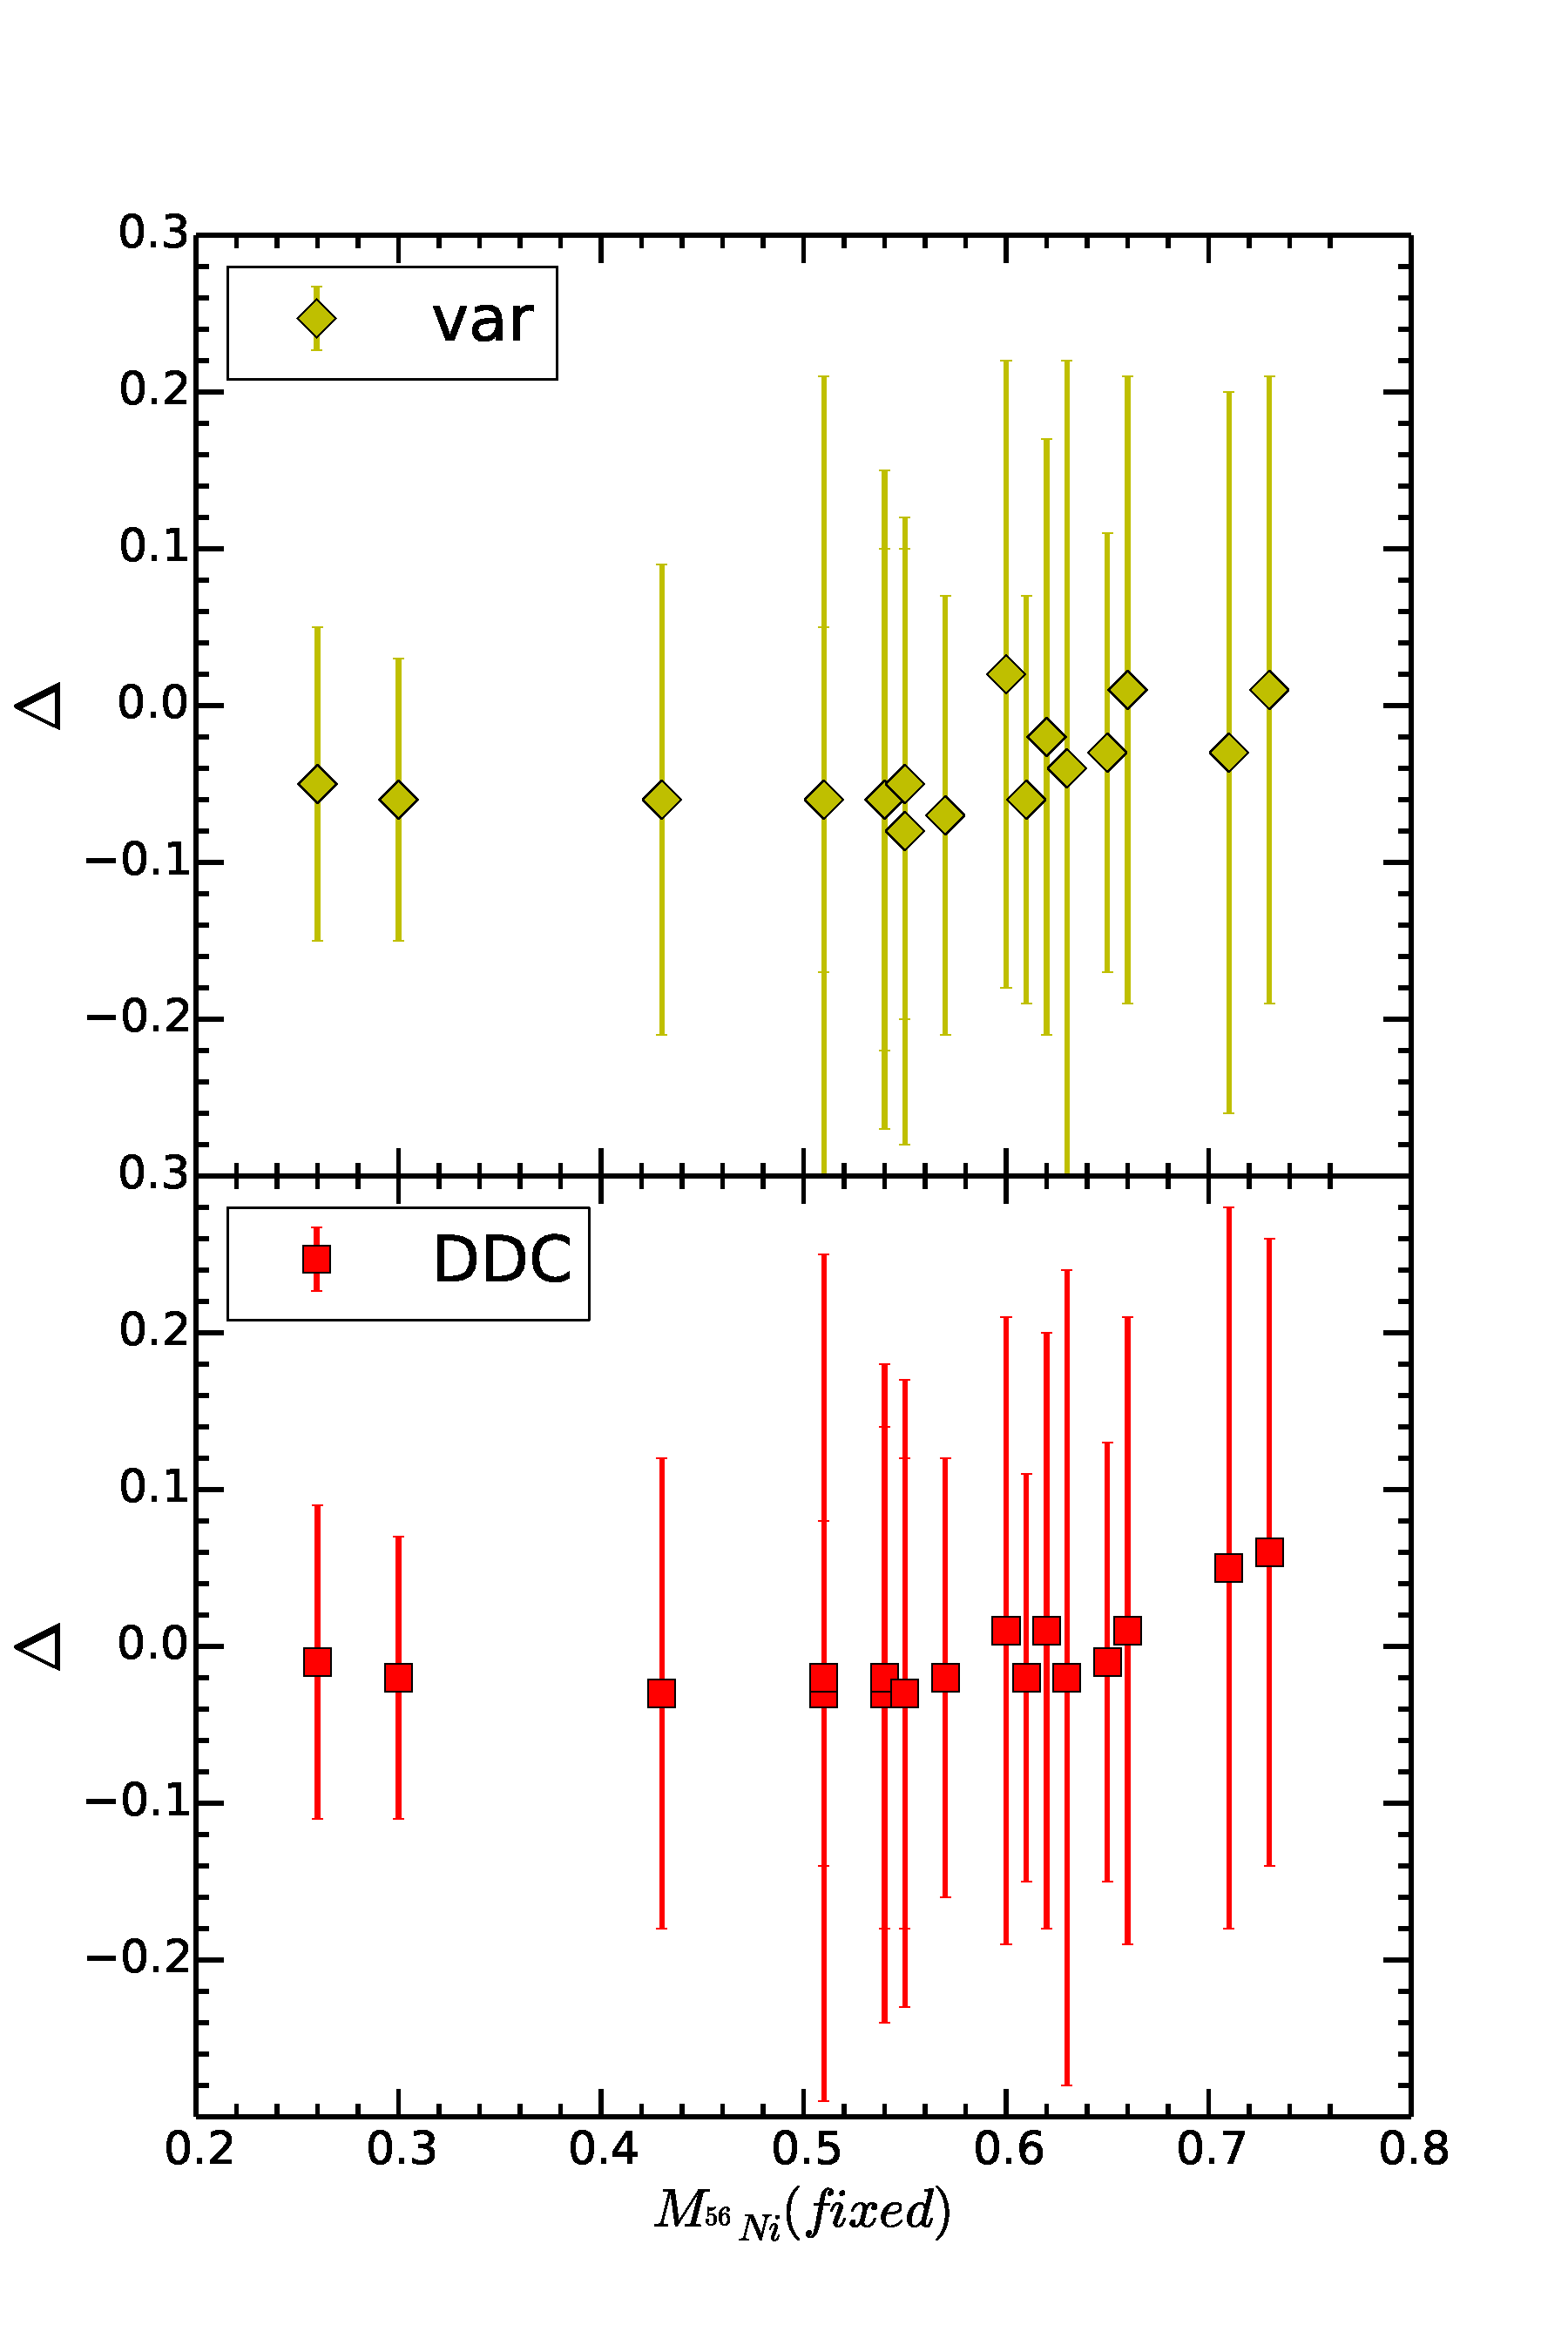
\includegraphics[width=.5\textwidth, trim= 0 30 0 30]{../plot_rel/dif_ni_comp.pdf}
\caption{\emph{Top}: The difference between the values estimated using a fixed rise time with Arnett's rule and the DDC models is plotted against the estimates from Arnett's rule with fixed rise time. \emph{Bottom}: The difference between values estimated using a fixed rise time with Arnett's rule and a variable rise time plotted against the estimates from Arnett's rule with fixed rise time. From the two panels we can see that the difference in the individual measurements are much smaller than the errors from a given method}
\label{fig:difarn}
\end{figure}

%---------------% 

\begin{figure}
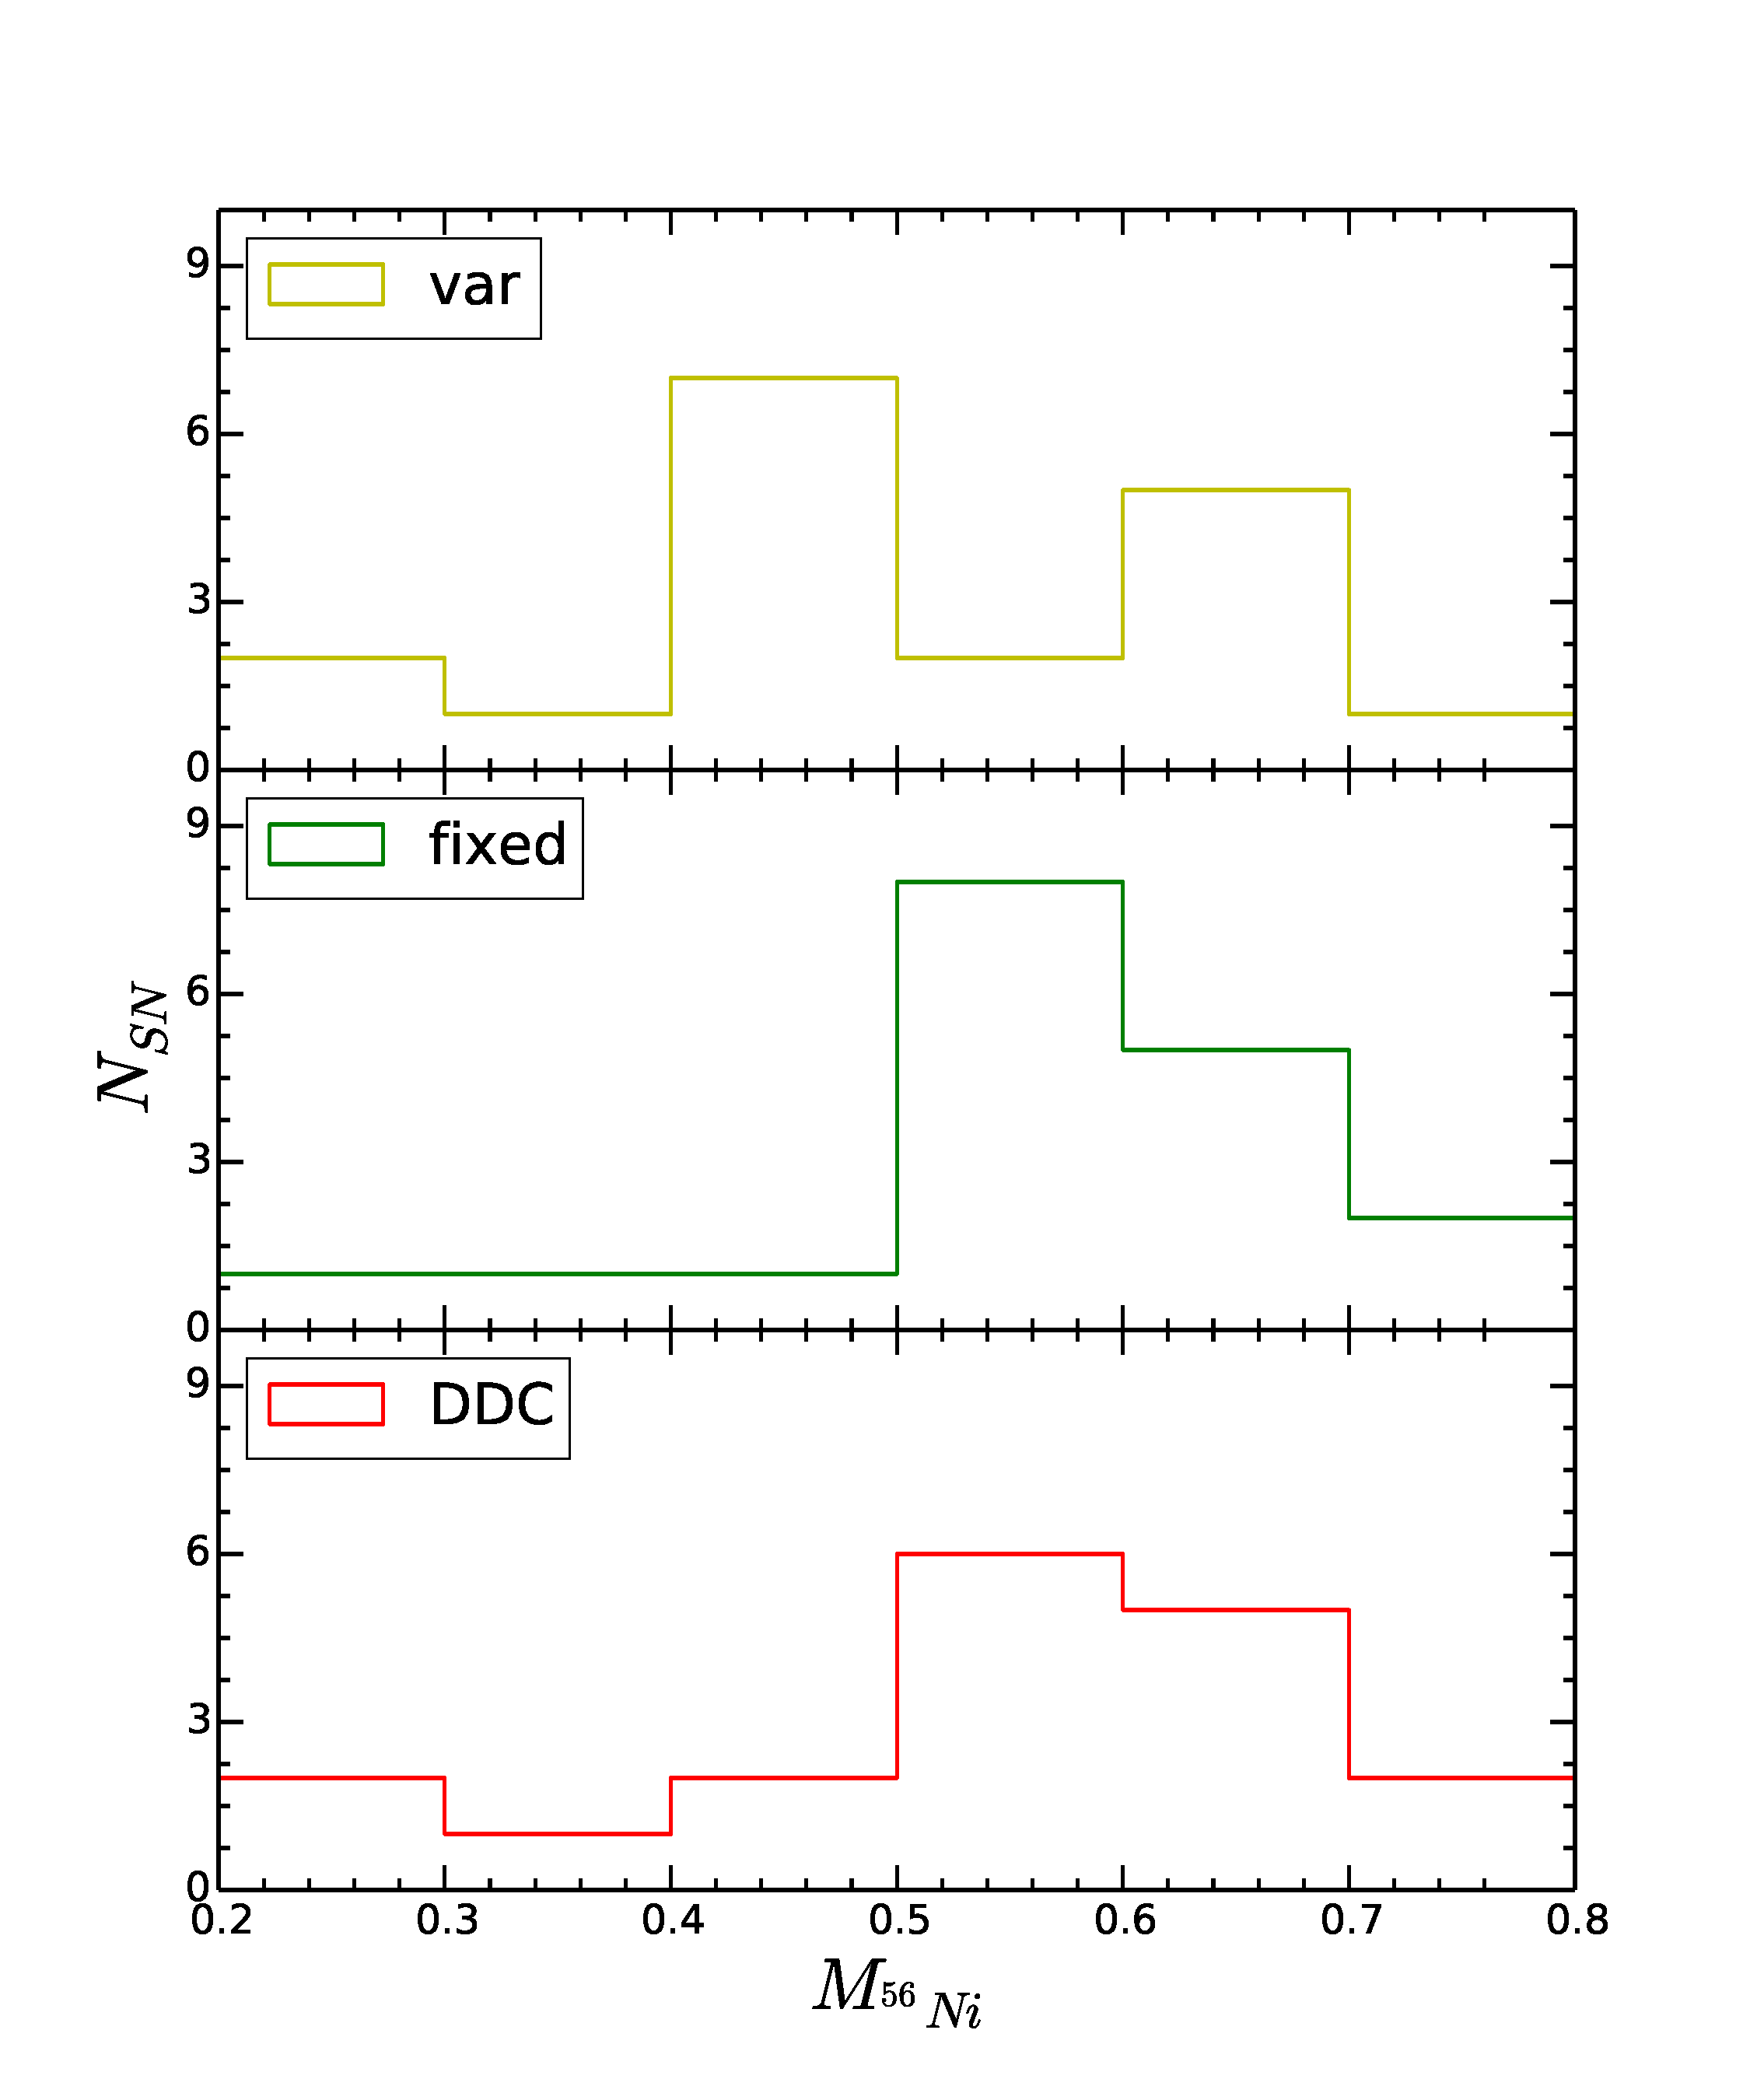
\includegraphics[width=.5\textwidth, trim= 0 30 0 30]{../plot_rel/hist_ni.pdf}
\caption{The histograms show the different methods to estimate the $M_{^{56}Ni}$ from the $L_{max}$. The values from Arnett's rule with fixed and variable rise time are plotted in the \emph{top} and \emph{middle} panels. The \emph{bottom} panel has the values estimated from the DDC models}
\label{fig:nicomp}
\end{figure}


Similar to previous studies we find that there is a large distribution in the $M_{^{56}Ni}$ values for the sample in Table \ref{tab:lr}. We note a factor of $\sim$ 3 difference between the lowest and highest $M_{^{56}Ni}$ values. We note that this sample doesn't include faint, 91bg-like objects, since their NIR light curves don't show a second maximum. These objects are seen to have a much lower $M_{^{56}Ni}$ $\sim$ 0.1 $M_{\odot}$. Thus, the complete distribution of $M_{^{56}Ni}$ for SNIa is expected to be wider than is seen in our sample.

%------------%


\subsection{Test Case for heavily reddened SNe}
Using the correlations derived above, we want to estimate the Ni masses of heavily reddened SNae. The first test case is the nearby SN 2014J in M82 with an $E(B-V)_{host}$ of 1.3. 
Current attempts to use the bolometric light curve depend on the $A_V$ value used and vary by a factor of $\sim$ 2
 (0.37 $M_{\odot}$ if using $A_V$=1.7 mag from \citet{Margutti2014}, compared to 0.77 using a higher $A_V$ of 2.5 mag from \citet{Goobar2014}).  In our analyses the aim is to 
 estimate the $M_{^{56}Ni}$ independent of the extinction.

The proximity of SN2014J, has allowed for the first $\gamma$ ray Co line detection in an SNIa (Churazov+ 2014). the authors, using a line photon escape fraction from the models, 
deduce an Ni mass of 0.62  $\pm$ 0.13 $M_{\odot}$. This provides a direct measurement of  $M_{^{56}Ni}$ for the SN. However, $\gamma$ ray detections aren't possible for farther away SN, for which we require a different estimation method. 

Using the best fit relation for the sample defined above , we obtain $M_{^{56}Ni}$ of 0.66 $\pm$ 0.15 $M_{\odot}$  for a $t_2$ of 31.99 $\pm$ 1.15 days. 
Thus, we find a very good correspondence between the values from the $\gamma$ rays and the NIR second maximum. This adds evidence to the argument that the NIR can be used for estimate $M_{^{56}Ni}$ for highly reddened SN.

Since we find from the DDC models that $\alpha$ is not constant for different $M_{^{56}Ni}$ (and hence, $L_{max}$) values, we use $\alpha$ corresponding to the peak luminosity of SN2014J. We do not find a significant change in the estimated $M_{^{56}Ni}$. Hence, for further analyses, we use $\alpha$=1

\begin{table*}
\begin{center}
\caption{Comparison of different methods to estimate $M_{^{56}Ni}$ for SN2014J}
\begin{tabular}{llcrr}
\hline
 $M_{Ni}$ (inferred) & $\sigma$ & Method & Reference\\
\hline
0.62	& 0.13 & $\gamma$ ray lines & \citet{Churazov2014} \\
0.37	& -- & Bolometric light curve $A_V$=1.7 mag &  \citet{Churazov2014, Margutti2014} \\
0.77	& -- & Bolometric light curve $A_V$=2.5 mag & \citet{Churazov2014, Goobar2014} \\
0.64	& 0.12 & NIR second maximum & this work \\

\hline
\end{tabular}
\end{center}
\label{tab:meth}
\end{table*}


For SN2014J, we can get a precise measurement of the extinction from IR spectra at $\sim$ +300 days ({\bf explain in greater detail}). This is again not possible for 
objects farther away. Thus, we apply this relation to a farther away, heavily extinguished object, SN2006X. 
The measured value for SN2006X of $t_2(J)$ is 28.19 with an error of 0.49  days. This results in an $M_{^{56}Ni}$ value of 0.58 $\pm$ 0.13 $M_{\odot}$. This value is consistent with the conclusion that SN2006X is a 'normal' SNIa \citep{Wang2008}. We compare this value for SN2006X to that obtained using $t_2(Y)$ and obtain $M_{^{56}Ni}$ of 0.58 $\pm$ 0.14 $M_{\odot}$. We find both these values consistent with each other. The slightly higher error bar on
 the value from $t_2(Y)$ is due to a larger error on the 
intercept in the best fit relation for the $Y$ band. 


In \citet{Wang2008}, the authors use multi-band photometry to correct the light curves for absorption from host galaxy dust. They derive a bolometric peak luminosity of 1.02 ($\pm$ 0.1) $\cdot e43$ $erg s^{-1}$. From $R$ band photometry, they derive a rise time to $B$ maximum of 18.2 $\pm$ 0.9d. Using this value in the expression for Arnett's rule, they derive a value of $M_{^{56}Ni}$= 0.50 $\pm$ 0.05 $M_{\odot}$. Thus, we conclude that the value derived from $t_2$ is consistent with published  $M_{^{56}Ni}$ values.   


\begin{table*}



\begin{center}
\caption{$M_{Ni}$ estimates for 5 objects with high values of $E(B-V)_{host}$. We present constraints from the relation using only $t_2(J)$ as well as from both $t_2(Y)$ and $t_2(J)$. We can see a marked decrease in the error values when combined constraints are used}
\begin{tabular}{llcccrr}
\hline
SN & $t_2(J)$ & $M_{Ni}$ (inferred) & $\sigma$ & $\mu$ & $e_{\mu}$ & Method \\
\hline
SN1986G	& 16.40 ($\pm$ 1.4)	&	0.32 & 0.10	& 28.01 & 0.12 & $J$ band relation \\
-- & --	& 0.33	& 0.08	&--&--& combined fit \\
SN2005A	& 27.58 ($\pm$ 0.3)	& 0.57	&  0.13 & 34.51 & 0.11  & $J$ band relation \\
-- & -- &	0.57	& 0.11	&--&--& combined fit \\
SN2006X	& 28.19  ($\pm$ 0.5)	& 0.57 & 0.13 &	 30.91 & 0.08 & $J$ band relation \\
-- & -- &	0.58	& 0.11	&--&--& combined fit \\
SN2008fp & 31.03 ($\pm$ 0.3)	& 0.64	& 0.15 & 31.79 & 0.05 & $J$ band relation \\
-- 	- &-- & 0.64	& 0.13	&--&--& combined fit		\\
SN2014J	& 31.99 ($\pm$ 1.2)	& 0.66	& 0.15 &  27.64 & 0.10   & $J$ band relation\\
--	& -- & 0.66  & 0.13 &--&--& combined fit \\
\hline
\end{tabular}

\label{tab:red}

\end{center}




\end{table*}



We include three more objects in the highly reddened SNe sample, namely, 1986G, 2005A and 2008fp. We calculate the $M_{^{56}Ni}$ for these objects in the same way as for SN2014J and SN2006X. We summarise our findings in Table ~\ref{tab:red}.
We can see that 1986G has a lower value of $M_{^{56}Ni}$ than the other objects in the sample. This is consistent with the observed optical decline rate and lower $B$ band luminosity of the SN. Since we find that $t_2$ in both $Y$ and $J$ bands correlates very strongly with the $M_{^{56}Ni}$, we use combined constraints from the relations to obtain an $M_{^{56}Ni}$ estimate.

% We can see from Table ~\ref{tab:red} that the error on the $M_{^{56}Ni}$ reduces when using combined constraints. For 2014J, it is 0.17 $M_{\odot}$ whereas for the others it is much lower at 0.07 $M_{\odot}$ 


Hence, we conclude that the NIR second maximum timing (in $Y$ and $J$) is a very good indicator of the amount of Nickel synthesised in the explosion, even for heavily reddened objects. 


\subsubsection{Combined fit}
From our analyses, we've found that the $t_2$ in $Y$ and $J$ is very strongly correlated to the $L_{max}$. In table \ref{tab:coeff}, we see that the slope values for the two bands is nearly identical and the intercepts are within the error bars. This prompted us to combine the information from the two bands for extrapolating the values of $L_{max}$ for objects not in the 'low-reddening' sample.

For the five objects listed above which have a very high $A_V$, we used the $J$ band relation to obtain an $M_{^{56}Ni}$. We also used a combined fit to the $Y$ and $J$ band data to evaluate the reduction in the error bar. For this, we presume that the $Y$ band estimate is equivalent to the value in the $J$ band, and hence, we calculate the slope and intercept with a greater number of data points, which leads to a reduction in the errors on the parameter estimates.  

\subsection{Complete NIR Sample}
Since we have derived the relation between $L_{max}$ and $t_2$, we evaluate the $L_{max}$ for all objects with a measured $t_2$ independent of the reddening estimates.
Since the slope for the relation in the $Y$ and $J$ bands is very similar and the intercepts are within error bars, we take the mean value for the slope and intercepFt as a 'combined' relation. We use the higher error on the intercept (from the $Y$ band) for the combined equation. We then use this to compare the estimates of $L_{max}$ from the $t_2$ in the two bands. In figure \ref{fig:yjcomp}, we plot the difference in the $L_{max}$ from the $t_2$ in $J$ and $Y$ against the $L_{max}$ estimated from $t_2(J)$. The difference in the two estimates is smaller than the error on the measurement. We note that the largest difference is for SN2005na, which has a $t_2(J)$ of 32.59, but a much smaller $t_2(Y)$ of 27.54. However, even for this object, the error is higher than the difference between the measurements   
%and have presented the different ways to obtain the $M_{Ni}$ from the $L_{max}$, we can then use the distribution of $t_2$ for all objects, independent of reddening to obtain a distribution of $M_{^{56}Ni}$ using the relations derived


\begin{figure}
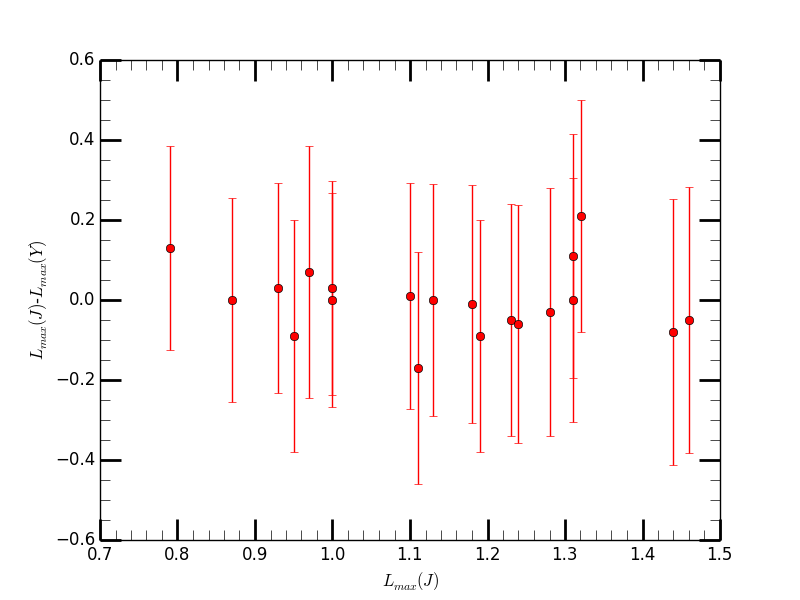
\includegraphics[width=.5\textwidth, height=0.25\textheight, trim= 0 30 0 30]{../plot_rel/lbol_comp_yj.png}


\caption{A comparison of the $L_{max}$ from the $t_2$ values measured in the $Y$ and $J$ bands. Plotted on the x-axis is the $L_{max}$ measured from $t_2(J)$ and on the y-axis is the difference between $L_{max}(J)$ and $L_{max}(Y)$. We can see that there is no trend between the two. The difference has a standard deviation of 0.08 ($\cdot$ $1e^{43}$) $erg s^{-1}$. The errors on each are errors in the individual measurements added in quadrature. We can see that the difference is smaller than the error. }
\label{fig:yjcomp}
\end{figure}

In section \ref{ssec-derni}, we have described the different methods for obtaining $M_{^{56}Ni}$ from $L_{max}$. Hence, we can derive a distribution for $M_{^{56}Ni}$ from the evaluated $L_{max}$ for the complete sample. 
\begin{figure}
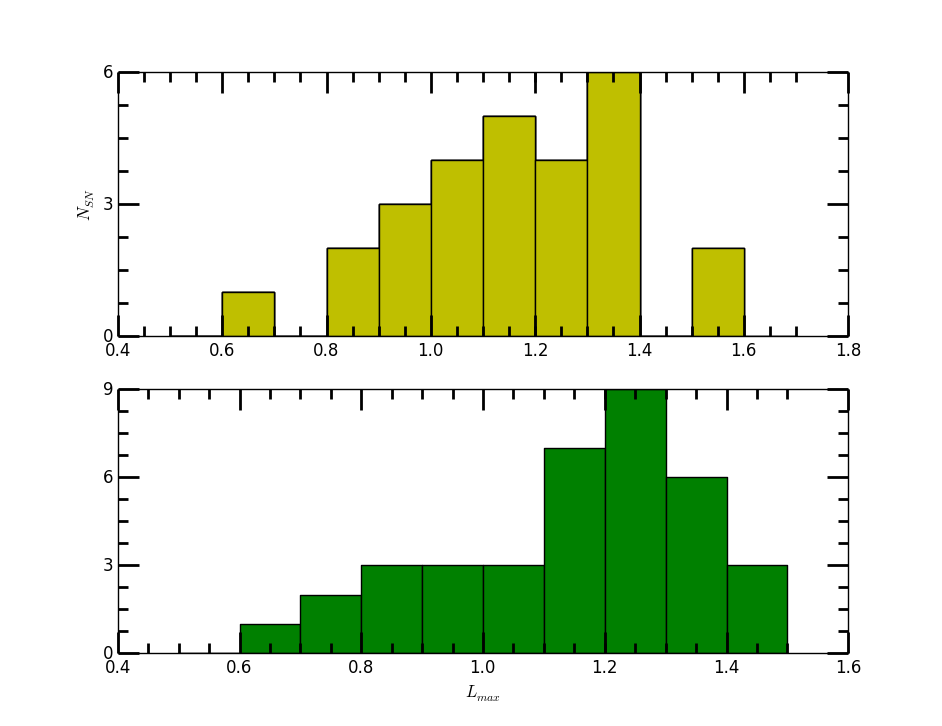
\includegraphics[width=.5\textwidth, trim= 0 30 0 30]{../plot_rel/lbol_yj_compsamp.png}
\caption{Histogram distributions of $L_{max}$ derived from the relations for the complete sample of objects (without the low reddening sample). \emph{Top}: Using the $t_2(Y)$ and \emph{bottom}: Using the $t_2(J)$. A large distribution in the $L_{max}$ values can be seen}
\label{fig:hist}
\end{figure}


In figure \ref{fig:hist} we plot the distribution of $M_{^{56}Ni}$ calculated from the $L_{max}$. We use Arnett's rule with a fixed rise time to get the $M_{^{56}Ni}$ from the $L_{max}$. From figure \ref{fig:hist}, we find a large scatter in the $M_{^{56}Ni}$ values. We find that the objects vary by a factor of 3 in their $M_{^{56}Ni}$ distribution. We note, however, that since faint, 91bg-like objects do not show a second maximum, we do not have values in the figure $\lesssim$ 0.2 $M_{\odot}$, hence, the expected variation for the complete population of SNIa is greater.  


\begin{table}
\begin{minipage}{70mm}
\begin{center}
\footnotetext{$^a$:$\cdot e^{43} erg s^{-1}$}
\caption{$M_{Ni}$ measurements for the complete sample of objects with $t_2$ measurements in both $Y$ and $J$ bands.}
\begin{tabular}{llcrr}
\hline
SN & $L_{max}^{a}$ (J)	& $\sigma$ & $L_{max}^{a}$ (Y) & $\sigma$ \\
\hline
1980N & 0.91 & 0.13 &\ldots & \ldots \\
1981B & 1.32 & 0.15 &\ldots & \ldots\\
1986G & 0.64 & 0.09 &\ldots & \ldots\\
1998bu & 1.23 & 0.14 &\ldots & \ldots\\
1999ac & 1.12 & 0.14 &\ldots & \ldots\\
1999ee & 1.42 & 0.16 &\ldots & \ldots \\
2000E & 1.31 & 0.16 &\ldots & \ldots\\
2000bh & 1.37 & 0.15 &\ldots & \ldots\\
2001bt & 1.17 & 0.13 &\ldots & \ldots\\
2001cn & 1.24 & 0.14 &\ldots & \ldots\\
2001cz & 1.40 & 0.16 &\ldots & \ldots\\
2001el & 1.29 & 0.15 &\ldots & \ldots\\
2002bo & 1.12 & 0.13 &\ldots & \ldots\\
2003cg & 1.24 & 0.14 &\ldots & \ldots\\
2003hv & 0.92 & 0.12 &\ldots & \ldots \\
2004ey	&	1.21	&	0.19	&	1.31	&	0.20	\\
2004gs	&	0.93	&	0.16	&	0.91	&	0.16	\\
2004gu	&	1.46	&	0.22	&	1.54	&	0.22	\\
2005A	&	1.10	&	0.18	&	1.12	&	0.18	\\
2005al	&	1.05	&	0.18	&	1.04	&	0.18	\\
2005na	&	1.35	&	0.20	&	1.13	&	0.19	\\
2006D	&	1.05	&	0.18	&	1.01	&	0.18	\\
2006X	&	1.13	&	0.18	&	1.13	&	0.19	\\
2006ax	&	1.32	&	0.20	&	1.36	&	0.21	\\

2006et	&	1.33	&	0.22	&	1.35	&	0.20	\\
2006gt 	& 0.85 		& 0.11 &\ldots & \ldots\\
2006hb	&	0.79	&	0.17	&	0.72	&	0.15	\\
2006kf	&	1.01	&	0.17	&	1.07	&	0.10	\\
2007S	&	1.46	&	0.21	&	1.52	&	0.23	\\
2007af	&	1.22	&	0.19	&	1.23	&	0.19	\\
2007as	&	1.02	&	0.22	&	0.94	&	0.17	\\
2007bc  &\ldots & \ldots & 1.16 &  0.2 \\
2007bm	&	1.15	&	0.17	&	1.32	&	0.20	\\
2007ca  &\ldots & \ldots & 1.38 &  0.22 \\
2007if  &\ldots & \ldots & 1.34 & 0.22 \\
2007jg  &\ldots & \ldots & 1.12 & 0.2  \\
2007le	&	1.27	&	0.20	&	1.31	&	0.20	\\
2007nq	&	0.98	&	0.18	&	0.94	&	0.17	\\
2008C	&	1.33	&	0.21	&	1.23	&	0.19	\\
2008fp	&	1.28	&	0.20	&	1.33	&	0.21	\\
2014J & 1.32 & 0.18 &\ldots & \ldots \\
\hline
\end{tabular}
\end{center}
\end{minipage}
\label{tab:yj}
\end{table}


In table \ref{tab:comp_ni}, we present the  $M_{^{56}Ni}$ values for the complete sample of objects with a measured $t_2(J)$ value. 




\iffalse
\begin{figure}
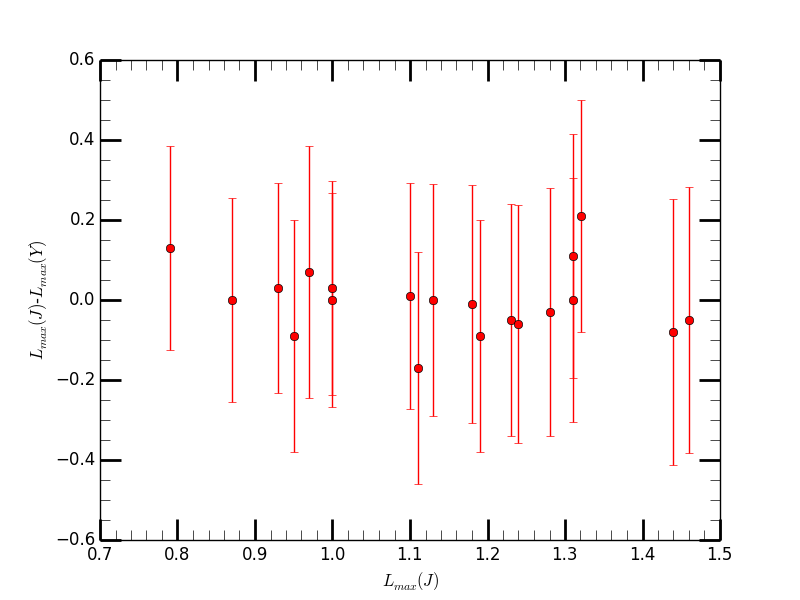
\includegraphics[width=.5\textwidth, trim= 0 30 0 30]{../plot_rel/lbol_comp_yj.pdf}
\caption{The plot shows the difference in the $M_{^{56}Ni}$ measured using $Y$ and $J$ band data, plotted against the $M_{^{56}Ni}$ measured from the $J$ band data. The mean value of the difference is 0.03 $M_{\odot}$ with a standard deviation of 0.037 $M_{\odot}$ (error bars on the x-axis have not been plotted for better visibilty of points)}
\label{fig:yjcomp}
\end{figure}
\fi

In figure \ref{fig:yjcomp}, we plot the difference between the $L_{max}$ estimated from the $t_2$ in $Y$ and $J$ bands against the $L_{max}$ estimated from $t_2(J)$ (called $L_{max}(J)$ in the figure). We find that there is no relation between the two quantities. The mean difference is 0.06 $M_{\odot}$ with a standard deviation of 0.05 $M_{\odot}$. This is lower than the error estimate on the individual values, which can be seen in the figure. 	


\subsection{Comparison with published values}
We searched the literature for published values of $M_{^{56}Ni}$ for objects in our sample. In \citet{Scalzo2014} , the authors published values of $M_{^{56}Ni}$ for 2005el and 2011fe. For 2011fe, we find $M_{^{56}Ni}$ of 0.52 $\pm$ 0.15 $M_{\odot}$ whereas the value in S14 is 0.42 $\pm$ 0.08. We note that the value of $\alpha$ in their study is 1.2 whereas we use $\alpha$=1. Using their value of $\alpha$, we find $M_{^{56}Ni}$= 0.44 $M_{\odot}$, which is a better agreement. SN2011fe also has a publsihed $M_{^{56}Ni}$ value in \cite{Pereira2013}, where the authors use different values of $\alpha$. For $\alpha$=1 they report a value of 0.53 $\pm$ 0.11 $M_{\odot}$, which agrees well with the value in this work. 

For SN2005el we find $M_{^{56}Ni}$ of 0.46 $\pm$ 0.11 $M_{\odot}$. S14 provides a discussion of this object, which in their sample they measure to have an  $M_{^{56}Ni}$ of 0.52. It is one of two outliers in their $M_{^{56}Ni}$-$\Delta m_{15}$. They argue that it is likely for the SN to have a lower $M_{^{56}Ni}$ that their fiducial analysis suggests.  






























\section{Discussion and Conclusion}
\label{sec-dnc}
In our sample, we observe a strong correlation between the $M_{Ni}$ and $t_2$ in $Y$ and $J$, and less so in the $H$ band. 
This provides us with direct evidence that the timing of the second maximum is governed by the amount of Nickel produced by the supernova
since it leads to a later ionization transition of the iron group elements at late time (mainly, $^{56}Co$) from doubly to singly ionized \citep{Kasen2006}.

This trend is confirmed by a strong correlation between  $t_L$  and $M_{Ni}$ indicating that objects with more Ni produced have a slower
rate of reddening and the Fe and Co lines appear later in the spectrum, which delays the onset of the lira law phase, and also the second maximum.

This relation offers great insight into measuring the $M_{Ni}$ for objects not in the low-reddening sample, but with extensive NIR data. 
A striking example of this application is the nearby SN2014J in M82, which is heavily occluded by host galaxy dust. Since this prevents 
an accurate measurement of $M_{Ni}$ from the bolometric light curves and there is a large disparity in the different values published in the literature
using this method, we use the relations we obtain to constrain the $M_{Ni}$. For SN2014J, we have a unique opportunity to compare different estimation methods, 
since its proximity has allowed $\gamma$ ray Co line detection and therefore, another extinction independent measurement of the $M_{Ni}$. Our value of 0.58 $\pm$ 0.21 $M_{odot}$
compares very well with \citet{Churazov2014}, who find $M_{Ni}$ of 0.61 $\pm$ 0.13 $M_{odot}$. The brightness of SN2014J at late times, due to its proximity, permits us to obtain
NIR spectra at $\sim$ 300 days, which can provide an accurate measurement of the extinction and therefore, an accurate $M_{Ni}$ from the bolometric light curve. This presents
us with a confrontation of several different methods to measure the $M_{Ni}$ and hence obtain a conclusive estimate on the amount of Ni produce in this SN.

Since $\gamma$ detections are unlikely for farther out SN and most of them are too faint at $\sim$ +300 days for IR spectroscopy, we apply our method to other heavily reddened SN
that are farther away than SN2014J. The first object we analyse is SN2006X. From the measurement of 0.57 $\pm$ 0.15 $M_{odot}$, we conclude that
2006X produced the average amount of Ni for an SNIa.

We also analyse the bolometric light curves at peak and during the late phase of exponential decline. We find that the SN in our sample have a uniform 
late time bolometric decline rate, indicating that the internal structure of the ejecta is similar for most SN. This confirms the deductions from the optical and NIR 
light curves in previous studies and from the bolometric light curves in sample of C00. We also find that the bolometric light curves, unlike the optical light curves,
have a narrow distribution of the $\Delta m_{15}$ parameter.  

We conclude from our findings that there is a strong dependence of the $t_2$ and the colour evolution (parametrized by $t_L$) on the $M_{Ni}$



%-------------------------------------%


\begin{acknowledgements}
This research was supported by the DFG Cluster of Excellence ʻOrigin and
Structure of the Universe'.
B.L. acknowledges support for this work by the Deutsche
Forschungsgemeinschaft through TRR33, The Dark Universe. We all are grateful to the ESO Visitor Programme to support the visit of S. B. to Garching when this work was started.
We would like to thank Rahman Amanullah for providing published photometry of SN2014J in the near infrared. 

\end{acknowledgements}

\begin{thebibliography}{99}
\bibitem[\protect\citeauthoryear{Ajhar et al.}{2001}]{Ajhar2001} 
Ajhar E.~A., Tonry J.~L., Blakeslee J.~P., Riess A.~G., Schmidt B.~P., 
2001, ApJ, 559, 584 

\bibitem[\protect\citeauthoryear{Amanullah et 
al.}{2014}]{Amanullah2014} Amanullah R., et al., 2014, ApJ, 788, 21

\bibitem[\protect\citeauthoryear{Arnett}{1982}]{Arnett1982} Arnett 
W.~D., 1982, ApJ, 253, 785 



\bibitem[\protect\citeauthoryear{Benetti et 
al.}{2004}]{Benetti2004} Benetti S., et al., 2004, MNRAS, 348, 261


\bibitem[\protect\citeauthoryear{Biscardi et 
al.}{2012}]{Biscardi2012} Biscardi I., et al., 2012, A\&A, 537, A57 

\bibitem[\protect\citeauthoryear{Blondin et 
al.}{2013}]{Blondin2013} Blondin S., Dessart L., Hillier D.~J., 
Khokhlov A.~M., 2013, MNRAS, 429, 2127 

\bibitem[\protect\citeauthoryear{Branch 
\& Tammann}{1992}]{Branch1992} Branch D., Tammann G.~A., 1992, ARA\&A, 30, 359 


\bibitem[\protect\citeauthoryear{Burns et al.}{2014}]{Burns2014} Burns
C.~R., et al., 2014, ApJ, 789, 32 

\bibitem[\protect\citeauthoryear{Cardelli, Clayton 
\& Mathis}{1989}]{Cardelli1989} Cardelli J.~A., Clayton G.~C.,
Mathis J.~S., 1989, ApJ, 345, 245 

\bibitem[\protect\citeauthoryear{Cartier et 
al.}{2014}]{Cartier2013} Cartier R., et al., 2014, ApJ, 789, 89

\bibitem[\protect\citeauthoryear{Churazov et 
al.}{2014}]{Churazov2014} Churazov E., et al., 2014, Natur, 
512, 406

\bibitem[\protect\citeauthoryear{Contardo, Leibundgut 
\& Vacca}{2000}]{Contardo2000} Contardo G., Leibundgut B., Vacca W.~D., 2000, A\&A, 359, 876 

\bibitem[\protect\citeauthoryear{Contreras et 
al.}{2010}]{Contreras2010} Contreras C., et al., 2010, AJ, 139, 519 

\bibitem[\protect\citeauthoryear{Diehl et al.}{2014}]{Diehl2014a} 
Diehl R., et al., 2014, arXiv, arXiv:1407.3061 

\bibitem[\protect\citeauthoryear{Diehl et al.}{2014}]{Diehl2014b} 
Diehl R., et al., 2014, arXiv, arXiv:1409.5477 

\bibitem[\protect\citeauthoryear{Filippenko et
al.}{1992}]{Filippenko1992} Filippenko A.~V., et al., 1992, AJ, 104,
1543 

\bibitem[\protect\citeauthoryear{Folatelli et 
al.}{2010}]{Folatelli2010} Folatelli G., et al., 2010, AJ, 139, 120 

\bibitem[\protect\citeauthoryear{Foley et 
al.}{2014}]{Foley2014} Foley R., et al., 2014, arXiv, 
arXiv:1405.3677

\bibitem[\protect\citeauthoryear{Freedman et 
al.}{2001}]{Freedman2001} Freedman W.~L., et al., 2001, ApJ, 553, 47 

\bibitem[\protect\citeauthoryear{Friedman et 
al.}{2014}]{Friedman2014} Friedman A.~S., et al., 2014, arXiv, 
arXiv:1408.0465 

\bibitem[\protect\citeauthoryear{Ganeshalingam, Li, 
\& Filippenko}{2011}]{G11} Ganeshalingam M., Li W., Filippenko A.~V., 2011, MNRAS, 416, 2607 


\bibitem[\protect\citeauthoryear{Goobar 
\& Leibundgut}{2011}]{Goobar2011} Goobar A., Leibundgut B., 2011, ARNPS, 61, 251

\bibitem[\protect\citeauthoryear{Goobar et al.}{2014}]{Goobar2014} 
Goobar A., et al., 2014, ApJ, 784, L12 


\bibitem[\protect\citeauthoryear{Hillebrandt 
\& Niemeyer}{2000}]{Hillebrandt2000} Hillebrandt W., Niemeyer J.~C., 2000, ARA\&A, 38, 191 

\bibitem[\protect\citeauthoryear{H\"oflich, Khokhlov \&
Wheeler}{1995}]{Hoeflich1995} H\" oflich P., Khokhlov A., Wheeler C.,
1995, ASPC, 73, 441 


\bibitem[\protect\citeauthoryear{Jack, Hauschildt, 
\& Baron}{2012}]{Jack2012} Jack D., Hauschildt P.~H., Baron E., 2012, A\&A, 538, A132 

\bibitem[\protect\citeauthoryear{Jensen et
al.}{2003}]{Jensen2003} Jensen J.~B., Tonry J.~L., Barris
B.~J., Thompson R.~I., Liu M.~C., Rieke M.~J., Ajhar E.~A., Blakeslee
J.~P., 2003, ApJ, 583, 712 

\bibitem[\protect\citeauthoryear{Jha, Riess, 
\& Kirshner}{2007}]{Jha2007} Jha S., Riess A.~G., Kirshner R.~P., 2007, ApJ, 659, 122 

\bibitem[\protect\citeauthoryear{Kasen}{2006}]{Kasen2006} Kasen 
D., 2006, ApJ, 649, 939

\bibitem[\protect\citeauthoryear{Kasen 
\& Woosley}{2007}]{Kasen2007} Kasen D., Woosley S.~E., 2007, ApJ, 656, 661 
 
\bibitem[\protect\citeauthoryear{Kattner et 
al.}{2012}]{Kattner2012} Kattner S., et al., 2012, PASP, 124, 114 

\bibitem[\protect\citeauthoryear{Krisciunas et 
al.}{2001}]{K01} Krisciunas K., et al., 2001, AJ, 122, 1616 

\bibitem[\protect\citeauthoryear{Krisciunas et 
al.}{2003}]{K03} Krisciunas K., et al., 2003, AJ, 125, 166 

\bibitem[\protect\citeauthoryear{Krisciunas et 
al.}{2004}]{K04a} Krisciunas K., et al., 2004a, AJ, 127, 1664 

\bibitem[\protect\citeauthoryear{Krisciunas et 
al.}{2004}]{K04b} Krisciunas K., et al., 2004b, AJ, 128, 3034 

\bibitem[\protect\citeauthoryear{Krisciunas et 
al.}{2007}]{K07} Krisciunas K., et al., 2007, AJ, 133, 58 

\bibitem[\protect\citeauthoryear{Krisciunas et 
al.}{2009}]{Krisciunas2009} Krisciunas K., et al., 2009, AJ, 138, 1584 

\bibitem[\protect\citeauthoryear{Kromer 
\& Sim}{2009}]{Kromer2009} Kromer M., Sim S.~A., 2009, MNRAS,
398, 1809 

\bibitem[\protect\citeauthoryear{Leaman et al.}{2011}]{Leaman2011} 
Leaman J., Li W., Chornock R., Filippenko A.~V., 2011, MNRAS, 412, 1419 

\bibitem[\protect\citeauthoryear{Leibundgut}{1988}]{Leibundgut1988} Leibundgut B., 1988, PhD thesis, University of Basel

\bibitem[\protect\citeauthoryear{Leibundgut}{2000}]{Leibundgut2000} Leibundgut B., 2000, A\&ARv, 10, 179 

\bibitem[\protect\citeauthoryear{Leibundgut}{2001}]{Leibundgut2001} Leibundgut B., 2001, ARA\&A, 39, 67 

\bibitem[\protect\citeauthoryear{Leibundgut et 
al.}{1993}]{Leibundgut1993} Leibundgut B., et al., 1993, AJ, 105,
301 

\bibitem[\protect\citeauthoryear{Leloudas et 
al.}{2009}]{Leloudas2009} Leloudas G., et al., 2009, A\&A, 505, 265 

\bibitem[\protect\citeauthoryear{Li et al.}{2001}]{Li2001} Li W., et
al., 2001, PASP, 113, 1178 

\bibitem[\protect\citeauthoryear{Li et al.}{2003}]{Li2003} Li W., et
al., 2003, PASP, 115, 453 

\bibitem[\protect\citeauthoryear{Lira}{1996}]{Lira1996} Lira P., 
1996, MsT, 3 

\bibitem[\protect\citeauthoryear{Maeda et al.}{2010}]{M10} 
Maeda K., Taubenberger S., Sollerman J., Mazzali P.~A., Leloudas G., Nomoto 
K., Motohara K., 2010, ApJ, 708, 1703 

\bibitem[\protect\citeauthoryear{Maeda et al.}{2011}]{M11} 
Maeda K., et al., 2011, MNRAS, 413, 3075 
\bibitem[\protect\citeauthoryear{Maguire et 
al.}{2012}]{Maguire2012} Maguire K., et al., 2012, MNRAS, 426, 2359 

\bibitem[\protect\citeauthoryear{Marion et al.}{2009}]{Marion2009} 
Marion G.~H., H{\"o}flich P., Gerardy C.~L., Vacca W.~D., Wheeler J.~C., 
Robinson E.~L., 2009, AJ, 138, 727 

\bibitem[\protect\citeauthoryear{Mandel et al.}{2009}]{Mandel2009} 
Mandel K.~S., Wood-Vasey W.~M., Friedman A.~S., Kirshner R.~P., 2009, ApJ, 
704, 629

\bibitem[\protect\citeauthoryear{Margutti et 
al.}{2014}]{Margutti2014} Margutti R., Parrent J., Kamble A., 
Soderberg A.~M., Foley R.~J., Milisavljevic D., Drout M.~R., Kirshner R., 
2014, ApJ, 790, 52

\bibitem[\protect\citeauthoryear{Mazzali et 
al.}{1997}]{Mazzali1997} Mazzali P.~A., Chugai N., Turatto M., Lucy 
L.~B., Danziger I.~J., Cappellaro E., della Valle M., Benetti S., 1997, 
MNRAS, 284, 151 

\bibitem[\protect\citeauthoryear{Mazzali et 
al.}{1998}]{Mazzali1998} Mazzali P.~A., Cappellaro E., Danziger 
I.~J., Turatto M., Benetti S., 1998, ApJ, 499, L49 

\bibitem[\protect\citeauthoryear{Mazzali et 
al.}{2007}]{Mazzali2007} Mazzali P.~A., R{\"o}pke F.~K., Benetti 
S., Hillebrandt W., 2007, Sci, 315, 825 

\bibitem[\protect\citeauthoryear{Matheson et 
al.}{2012}]{Matheson2012} Matheson T., et al., 2012, ApJ, 754, 19 

\bibitem[\protect\citeauthoryear{Meikle}{2000}]{Meikle2000} Meikle 
W.~P.~S., 2000, MNRAS, 314, 782 

\bibitem[\protect\citeauthoryear{Nadyozhin}{1994}]{Nadyozhin1994} 
Nadyozhin D.~K., 1994, ApJS, 92, 527 

\bibitem[\protect\citeauthoryear{Nobili et 
al.}{2005}]{Nobili2005} Nobili S., et al., 2005, A\&A, 437, 789 

\bibitem[\protect\citeauthoryear{Nobili 
\& Goobar}{2008}]{Nobili2008} Nobili S., Goobar A., 2008, A\&A, 487, 19 

\bibitem[\protect\citeauthoryear{Pastorello et 
al.}{2007}]{Pastorello2007} Pastorello A., et al., 2007, MNRAS, 377, 
1531 

\bibitem[\protect\citeauthoryear{Patat et 
al.}{2013}]{Patat2013} Patat F., et al., 2013, A\&A, 549, A62 

\bibitem[\protect\citeauthoryear{Pereira et 
al.}{2013}]{Pereira2013} Pereira R., et al., 2013, A\&A, 554, A27 

\bibitem[\protect\citeauthoryear{Perlmutter et
al.}{1999}]{Perlmutter1999} Perlmutter S., et al., 1999, ApJ, 517, 565 

\bibitem[\protect\citeauthoryear{Phillips}{1993}]{Phillips1993} 
Phillips M.~M., 1993, ApJ, 413, L105 

\bibitem[\protect\citeauthoryear{Phillips}{2012}]{Phillips2012} 
Phillips M.~M., 2012, PASA, 29, 434 

\bibitem[\protect\citeauthoryear{Phillips et 
al.}{1999}]{Phillips1999} Phillips M.~M., Lira P., Suntzeff N.~B., 
Schommer R.~A., Hamuy M., Maza J., 1999, AJ, 118, 1766 

\bibitem[\protect\citeauthoryear{Phillips et 
al.}{2006}]{Phillips2006} Phillips M.~M., et al., 2006, AJ, 131, 
2615 

\bibitem[\protect\citeauthoryear{Phillips et 
al.}{2013}]{Phillips2013} Phillips M.~M., et al., 2013, ApJ, 779, 38 

\bibitem[\protect\citeauthoryear{Pignata et 
al.}{2008}]{Pignata2008} Pignata G., et al., 2008, MNRAS, 388, 971 

\bibitem[\protect\citeauthoryear{Pinto 
\& Eastman}{2000}]{Pinto2000} Pinto P.~A., Eastman R.~G., 2000, ApJ, 530, 757 

\bibitem[\protect\citeauthoryear{Riess, Press, 
\& Kirshner}{1996}]{Riess1996} Riess A.~G., Press W.~H., Kirshner R.~P., 1996, ApJ, 473, 88 

\bibitem[\protect\citeauthoryear{Riess et al.}{1998}]{Riess1998} 
Riess A.~G., et al., 1998, AJ, 116, 1009 

\bibitem[\protect\citeauthoryear{Scalzo et al.}{2010}]{Scalzo2010} 
Scalzo R., et al., 2010, ApJ, 713, 1073 
\bibitem[\protect\citeauthoryear{Scalzo et al.}{2012}]{Scalzo2012} 
Scalzo R., et al., 2012, ApJ, 757, 12 
\bibitem[\protect\citeauthoryear{Scalzo et al.}{2014}]{Scalzo2014} 
Scalzo R., et al., 2014, MNRAS, 560 



\bibitem[\protect\citeauthoryear{Stritzinger et
al.}{2006}]{Stritzinger2006} Stritzinger M., Leibundgut B., Walch S.,
Contardo G., 2006, A\&A, 450, 241 

\bibitem[\protect\citeauthoryear{Stritzinger et 
al.}{2011}]{Stritzinger2011} Stritzinger M.~D., et al., 2011, AJ, 142, 
156 
\bibitem[\protect\citeauthoryear{Suntzeff}{1996}]{Suntzeff1996} 
Suntzeff N.~B., 1996, ssr..conf, 41 
\bibitem[\protect\citeauthoryear{Tonry et al.}{2001}]{Tonry2001} 
Tonry J.~L., Dressler A., Blakeslee J.~P., Ajhar E.~A., Fletcher A.~B., 
Luppino G.~A., Metzger M.~R., Moore C.~B., 2001, ApJ, 546, 681

\bibitem[\protect\citeauthoryear{Tripp}{1998}]{Tripp1998} Tripp R., 1998, A\&A, 331, 815 

\bibitem[\protect\citeauthoryear{Tully}{1988}]{Tully1988} Tully 
R.~B., 1988, ngc..book,
\bibitem[\protect\citeauthoryear{Valentini et 
al.}{2003}]{Valentini2003} Valentini G., et al., 2003, ApJ, 595,
779 
\bibitem[\protect\citeauthoryear{Wang et al.}{2008}]{Wang2008} 
Wang X., et al., 2008, ApJ, 675, 626 
\bibitem[\protect\citeauthoryear{Weyant et al.}{2014}]{Weyant2014} 
Weyant A., Wood-Vasey W.~M., Allen L., Garnavich P.~M., Jha S.~W., Joyce 
R., Matheson T., 2014, ApJ, 784, 105 



\end{thebibliography}


%\appendix
%\section{Principal Component Analysis in the combined fit}

In section \ref{} we try to simultaneously fit the $t_2$ in $Y$ and $J$ to obtain combined constraints on $L_{max}$. However, the multivariate regression returns estimates with insignificant $t$-statistics and a high standard error. Moreover, the slope estimated for the $Y$ band $t_2$ is \emph{negative} which is incorrect since the $t_2(Y)$ has a positive correlation with $L_{max}$. 

These estimates for the multivariate regression are incorrect due to the problem of multicollinearity. This arsies due to the strong correlation between the predictor variables, in this case, $t_2$ $Y$ and $J$ In order to circumvent this problem, we apply a principal component analysis (PCA) to the two variables and transform them into uncorrelated principal components. 

We use  a Python package \emph{sci-kit learn} to decompose the variables into a principal component (PC). We derive a linear relation between the PC and the $L_{max}$ values in Table \ref{tab:mni}. 
The measured $t_2$ for heavily reddened objects are transformed in the direction of the PC and the error from the slope of the linear relation is propagated. For the final estimated $L_{max}$, we add the mean $L_{max}$ for the objects in the low-reddening sample. The error on the mean is calculated by bootstrap resampling.  
We find that the PCA estimates give a marginal improvement on the error 

\begin{table}
\begin{center}
\caption{$M_{Ni}$ estimates for 5 objects with high values of $E(B-V)_{host}$. We present constraints from the relation using only $t_2(J)$ as well as from both $t_2(Y)$ and $t_2(J)$. We can see a marked decrease in the error values when combined constraints are used}
\begin{tabular}{llcccrr}
\hline
SN &  $M_{Ni}$ (inferred) & $\sigma$  \\
\hline
SN1986G	& 0.34 & 0.08	\\
SN2005A	& 0.56	&  0.10  \\
SN2006X	& 0.57 & 0.10  \\\
SN2008fp &  0.63 & 0.11 \\
SN2014J	& 0.66	& 0.12 \\

\hline
\end{tabular}
\label{tab:pca_red}
\end{center}
\end{table}


\end{document}
 